\documentclass{article}
\usepackage[preprint]{colm2026_conference}

\usepackage[utf8]{inputenc}
\usepackage[T1]{fontenc}
\usepackage{hyperref}
\usepackage{url}
\usepackage{booktabs}
\usepackage{amsmath}
\usepackage{amssymb}
\usepackage{amsfonts}
\usepackage{graphicx}
\usepackage{nicefrac}
\usepackage{microtype}
\usepackage{xcolor}
\usepackage{placeins}
\usepackage{listings}
\usepackage{longtable}
\usepackage{xurl} % better URL line-breaking
\usepackage{lineno}

\usepackage{fontawesome5}

\usepackage{tikz}
\usetikzlibrary{arrows.meta,positioning,fit,calc,backgrounds}

\newcommand{\theHalgorithm}{\arabic{algorithm}}

\definecolor{darkblue}{rgb}{0, 0, 0.5}
\hypersetup{colorlinks=true, citecolor=darkblue, linkcolor=darkblue, urlcolor=darkblue}

\graphicspath{{figures/}}

% Listings setup for prompt blocks (two-column friendly, no boxes)
\lstset{
  basicstyle=\\ttfamily\\scriptsize,
  breaklines=true,
  breakatwhitespace=false, % allow breaking long tokens
  columns=fullflexible,
  keepspaces=true,
  showstringspaces=false,
  tabsize=2,
  frame=none,
  xleftmargin=0pt,
  xrightmargin=0pt,
  aboveskip=0.5em,
  belowskip=0.5em,
}

\title{Moral Susceptibility and Robustness under Persona Role-Play in Large Language Models}

\author{
Davi Bastos Costa, Felippe Alves, and Renato Vicente \\
TELUS Digital Research Hub, Center for Artificial Intelligence and Machine Learning \\
Institute of Mathematics, Statistics and Computer Science, University of S\~ao Paulo\\
\{davi.costa,\ felippe.pereira,\ rvicente\}@usp.br
}

\begin{document}

\ifcolmsubmission
\linenumbers
\fi


\maketitle

\begin{abstract}
  Large language models (LLMs) increasingly operate in social contexts, motivating analysis of how they express and shift moral judgments. In this work, we investigate the moral response of LLMs to persona role-play, prompting a LLM to assume a specific character. Using the Moral Foundations Questionnaire (MFQ), we introduce a benchmark that quantifies two properties: moral susceptibility and moral robustness, defined from the variability of MFQ scores across- and within-personas. We estimate these quantities with two complementary procedures, repeated sampling and a logit-based method that directly estimates the rating distributions and enables temperature analysis. We evaluate 15 models across six families: Claude, DeepSeek, Gemini, GPT, Grok, and Llama. The two metrics show qualitatively different patterns. Moral robustness varies by more than an order of magnitude, with a coefficient of variation of about $152\%$, and is explained almost entirely by model family. The Claude family is, by a significant margin, the most robust, about 30 times more so than the lower-performing families (DeepSeek, Grok, and Llama), while Gemini and GPT occupy an intermediate tier. This strong family dependence suggests that robustness is primarily shaped by post-training. Moral susceptibility, by contrast, spans a much narrower range, with a coefficient of variation of about $13\%$, and the most susceptible model is only 1.6 times more susceptible than the least. Unlike robustness, susceptibility shows no clear family dependence, suggesting that it is primarily determined by pre-training.  Additionally, we present moral foundation profiles for models without persona role-play and for personas averaged across models. Together, these analyses provide a systematic view of how persona conditioning shapes moral behavior in LLMs and a window into the internal machinery they use to instantiate personas.
\end{abstract}


\section{Introduction}
As large language models (LLMs) move into interactive, multi-agent settings, reliable benchmarks for their social reasoning are essential. Recent evaluations probe theory-of-mind, multi-agent interactions under asymmetric information, cooperation, and deception through controlled role-play and game-theoretic tasks \cite{zhou2024sotopia,pan2023machiavelli,bianchi2024negotiationarena,chen-etal-2024-tombench,costa2025deceivedetectdiscloselarge}. Complementary datasets benchmark social commonsense, moral judgment, and self-recognition capabilities \cite{sap-etal-2019-social,hendrycks2021ethics,bai2025knowthyselfincapabilityimplications}. Motivated by this landscape, we focus on moral judgment as a core facet of social decision-making and alignment.

This paper introduces a benchmark that combines persona role-play---prompting a LLM to assume a specific character---with the Moral Foundations Questionnaire \citep{moralfoundations2017questionnaires}, a widely used instrument in moral psychology that measures five moral foundations: Harm/Care, Fairness/Reciprocity, In-group/Loyalty, Authority/Respect, and Purity/Sanctity \citep{graham2009liberals,haidt2007when,moralfoundations2017questionnaires}. We elicit LLMs to respond to the MFQ while role-playing personas drawn from \citet{ge2025scalingsyntheticdatacreation}. From these responses, we define two complementary quantities: moral robustness, the within-persona stability of MFQ scores under repeated sampling (averaged across personas), and moral susceptibility, the sensitivity of MFQ scores to persona variation. Operationally, we estimate these quantities in two ways: the main benchmark uses repeated sampling, which applies uniformly across queried models, while a complementary logit-based procedure is available for models that expose next-token distributions and provides a more direct estimate of the induced rating distribution. See Fig.~\ref{fig:mfq-susceptibility-robustness} for a conceptual overview diagram. These metrics are defined in Eq.~\eqref{eq:robustness} and Eq.~\eqref{eq:overall-susceptibility}, each with foundation-level decompositions and uncertainty estimates. 

\begin{figure*}[t!]
  \centering
  \definecolor{suscolor}{HTML}{4A90E2} % Gemini palette
  \definecolor{robcolor}{HTML}{E67E22} % Claude-Sonnet palette
  \definecolor{promptcolor}{HTML}{4A90E2}
  \definecolor{modelcolor}{HTML}{E67E22}
  \definecolor{ratingcolor}{HTML}{52B788}
  \definecolor{datacolor}{HTML}{F9E79F}
  \definecolor{susbgcolor}{HTML}{BDA0E3}
  \resizebox{0.7\textwidth}{!}{%
  \begin{tikzpicture}[
    font=\small,
    node distance=12mm and 18mm,
    % styles
    box/.style = {draw, rounded corners, inner sep=6pt, align=left},
    persona/.style = {draw=modelcolor!50!black, rounded corners=3pt, inner xsep=6pt, inner ysep=3pt, align=left, text=black, fill=modelcolor!25},
    title/.style = {font=\bfseries},
    arrow/.style = {line width=1pt, -{Latex[length=2.4mm,width=1.4mm]}},
  ]

  % Persona stack (center)
  \matrix (pers) [column sep=0mm, row sep=2mm] {
    \node[persona] (p0) {\faUser\ \ Persona $0$}; \\
    \node[persona] (p1) {\faUser\ \ Persona $1$}; \\
    \node[inner ysep=3pt, inner xsep=2pt] (dots) {$\vdots$}; \\
    \node[persona] (plast) {\faUser\ \ Persona $|\mathcal{P}|$}; \\
  };

  % Susceptibility box around personas (background layer so text stays visible)
  \begin{pgfonlayer}{background}
    \node[draw=susbgcolor!70!black, rounded corners, fill=susbgcolor!40,
          fit=(p0) (p1) (dots) (plast), inner xsep=12pt, inner ysep=10pt,
          label={[title]above:Moral Susceptibility},
          label={[text=black]below:Across-persona variability}] (susbox) {};
  \end{pgfonlayer}

  % Data block (vertical)
  \node[draw=black, rounded corners, inner xsep=6pt, inner ysep=6pt, align=center, fill=datacolor!70, label={[title]above:Model}] (modelbox) [left=32mm of susbox] {
    \begin{tikzpicture}[scale=0.42, line width=0.45pt]
      \foreach \y [count=\i] in {0.75,-0.35,-1.45} {
        \node[draw,circle,inner sep=1.2pt] (in\i) at (0,\y) {};
      }
      \foreach \y [count=\i] in {0.75,-0.35,-1.45} {
        \node[draw,circle,inner sep=1.2pt] (hid\i) at (1,\y) {};
      }
      \foreach \y [count=\i] in {0.2,-0.9} {
        \node[draw,circle,inner sep=1.2pt] (out\i) at (2,\y) {};
      }
      \foreach \i in {1,2,3} {
        \foreach \j in {1,2,3} {
          \draw (in\i) -- (hid\j);
        }
      }
      \foreach \i in {1,2,3} {
        \foreach \j in {1,2} {
          \draw (hid\i) -- (out\j);
        }
      }
    \end{tikzpicture}
  };

  \node[draw=black, rounded corners, inner xsep=6pt, inner ysep=6pt, align=left, fill=promptcolor!18, label={[title]above:Prompt}] (promptbox) [above=10mm of modelbox] {
    \begin{tabular}{@{}l@{}}
      \strut \faUser\ Persona\\[4pt]
      \strut \faFile\ MFQ
    \end{tabular}
  };

  \node[draw=black, rounded corners, inner xsep=6pt, inner ysep=6pt, align=center, fill=ratingcolor!22, label={[title]above:MFQ Scores}] (scorebox) [below=14mm of modelbox] {
    \begin{tikzpicture}[x=3.8mm, y=4.8mm, baseline=(current bounding box.center)]
      \draw[black!55] (-0.2,0) -- (5.2,0);
      \foreach \x/\y in {0/0.08,1/0.34,2/0.78,3/0.78,4/0.34,5/0.08} {
        \draw[black!45] (\x,0.03) -- (\x,-0.07);
        \fill[ratingcolor!85!black] (\x,\y) circle (1.3pt);
        \node[font=\scriptsize, below=2pt] at (\x,-0.07) {$\x$};
      }
    \end{tikzpicture}
  };

  \coordinate (promptarrowstart) at ($(promptbox.south)+(0,-8pt)$);
  \coordinate (modelarrowend) at ($(modelbox.north)+(0,8pt)$);
  \coordinate (modelarrowstart) at ($(modelbox.south)+(0,-13pt)$);
  \coordinate (scorearrowend) at ($(scorebox.north)+(0,13pt)$);
  \draw[arrow] (promptarrowstart) -- (modelarrowend);
  \draw[arrow] (modelarrowstart) -- (scorearrowend);

  % Robustness box (right)
  \node[
    box,
    draw=robcolor,
    text=black,
    fill=modelcolor!14,
    right=28mm of susbox,
    anchor=center,
    inner xsep=8pt,
    inner ysep=8pt,
    align=center
  ] (runs) {%
    \begin{tikzpicture}[x=4.8mm, y=7mm, baseline=(current bounding box.center)]
      \draw[black!55] (-0.2,0) -- (6.2,0);
      \foreach \x/\y in {0/0.08,1/0.28,2/0.68,3/1.00,4/0.68,5/0.28,6/0.08} {
        \draw[black!45] (\x,0.03) -- (\x,-0.07);
        \fill[robcolor] (\x,\y) circle (1.6pt);
        \node[font=\scriptsize, below=2pt] at (\x,-0.07) {$\x$};
      }
      \draw[robcolor!80!black, line width=0.9pt, <->] (2,0.40) -- (4,0.40);
    \end{tikzpicture}
  };

  % Robustness title above runs
  \node[title, text=black, above=2mm of runs] {Moral Robustness};
  \node[text=black, below=2mm of runs] {Within-persona variability};

  % Merge point for persona arrows before entering robustness box
  \coordinate (merge) at ($(runs.center)+(-6mm,0)$);
  \coordinate (p0merge) at ($(p0.east)!0.60!(merge)$);
  \coordinate (p1merge) at ($(p1.east)!0.60!(merge)$);
  \coordinate (plastmerge) at ($(plast.east)!0.60!(merge)$);
  \coordinate (runsentry) at ($(runs.center)+(-1.5mm,0)$);

  % Persona arrows converge at merge point, leaving a small gap before merging
  \draw[arrow] (p0.east) -- (p0merge);
  \draw[arrow] (p1.east) -- (p1merge);
  \draw[arrow] (plast.east) -- (plastmerge);

  % Overall analysis grouping
  \coordinate (datatop) at ($(promptbox.north)+(0,6mm)$);
  \coordinate (databottom) at ($(scorebox.south)+(0,-6mm)$);

  \begin{pgfonlayer}{background}
    \node[draw=black, rounded corners, fit=(promptbox) (modelbox) (scorebox) (datatop) (databottom), inner xsep=8pt, inner ysep=0pt, label={[title]below:Data}] (databox) {};
    \node[draw=black, rounded corners, line width=0.9pt, fit=(susbox) (runs), inner xsep=28pt, inner ysep=26pt, label={[title]below:Benchmark}] (analysisbox) {};
  \end{pgfonlayer}


  \end{tikzpicture}%
  }% end \resizebox
  \caption{Left: summary of our data collection pipeline: we elicit models to respond to the MFQ conditioned on a persona. Right: summary of our benchmark pipeline: robustness, Eq.~\ref{eq:robustness}, and susceptibility, Eq.~\ref{eq:overall-susceptibility}, are computed from within and across persona variability in MFQ scores, respectively.}
  \label{fig:mfq-susceptibility-robustness}
\end{figure*}

  

Applying this framework across 15 models spanning six families, we find that moral robustness varies by more than an order of magnitude (coefficient of variation $\approx 152\%$), with this variation almost entirely accounted for by model family rather than size. We read this strong family dependence as evidence that robustness is primarily determined by post-training. Moral susceptibility behaves differently: it occupies a much narrower range (coefficient of variation $\approx 13\%$), shows no family dependence, and depends only mildly on size within families, consistent with susceptibility being primarily determined by pre-training. Among individual models, Claude Sonnet 4.5 is the most robust and Grok 4 Fast the least; Gemini 2.5 Flash is the most susceptible, while Llama 4 Scout is the least. Robustness and susceptibility are largely orthogonal at the model level (\(r \approx -0.03\)); the joint scatter reveals distinct family clusters rather than a monotonic trade-off, and foundation-level decompositions show that Purity/Sanctity is the only foundation where robustness and susceptibility are moderately negatively associated.

Recent research has examined the moral and social behavior of LLMs through the lens of the MFQ, exploring their value orientations, cultural variability, and alignment with human moral judgments \citep{abdulhai-etal-2024-moral,nunes2024hypocrites,aksoy2024whose,bajpai2024insights,ji2025moralbenchmoralevaluationllms}. Parallel efforts study persona role-playing as a mechanism for conditioning model behavior, including benchmarks, interactive environments, and diagnostic analyses \citep{tseng2024two,wang2023rolellm,samuel2025personagym,yu2025rpgbench,xu2024character,elboudouri2025rpeval,bai2025concept}. Our MFQ persona framework bridges these directions by systematically quantifying how persona conditioning alters moral judgments, separating the effects of repeated sampling (moral robustness) from those of persona variation (moral susceptibility). In addition, we report MFQ profiles for both unconditioned and persona-conditioned settings, providing a comparative view of baseline moral tendencies and persona-driven moral shifts across models.

\section{Moral Robustness and Susceptibility Benchmark}

We define a benchmark to evaluate the moral robustness and moral susceptibility of LLMs. Moral robustness measures the stability of MFQ ratings and moral susceptibility measures the sensitivity of MFQ scores to persona variation. These quantities are defined in Eq.~\eqref{eq:robustness} and Eq.~\eqref{eq:overall-susceptibility} respectively.

\subsection{Moral Foundation Questionnaire}

The Moral Foundations Questionnaire \citep{moralfoundations2017questionnaires} is a widely used instrument in moral psychology \citep{graham2009liberals,haidt2007when,moralfoundations2017questionnaires} and comprises 30 questions split into two sections. The first includes 15 relevance judgments, which assess how relevant certain considerations are when deciding what is right or wrong, and the second includes 15 agreement statements, which measure the level of agreement with specific moral propositions \citep{graham2011mfq,moralfoundations2017questionnaires}. In both sections, respondents answer each item using an integer scale from 0 to 5, representing in the first section the perceived relevance of the consideration and in the second the degree of agreement with the statement (see Appendix~\ref{app:prompts} for a verbatim description including the interpretation of the scale). Questions map to five moral foundations: Harm/Care, Fairness/Reciprocity, In-group/Loyalty, Authority/Respect, Purity/Sanctity. The results are typically presented as foundation-level scores, obtained by averaging the ratings of the questions associated with each foundation.

Figure~\ref{fig:mfq-profiles} illustrates the resulting foundation-level MFQ scores across models in the no-persona condition. Models were elicited to answer the 30 MFQ questions 10 times each, which we average by foundation and display as radar profiles with the corresponding standard error band. We show four representative models in the main text and defer the full one-radar-per-model collection to Appendix~\ref{app:moral-foundation-profile}. Although not the focus of our work, understanding the moral profile of different frontier models is relevant, providing useful context for deployment and comparison.

\begin{figure}[t!]
  \centering
  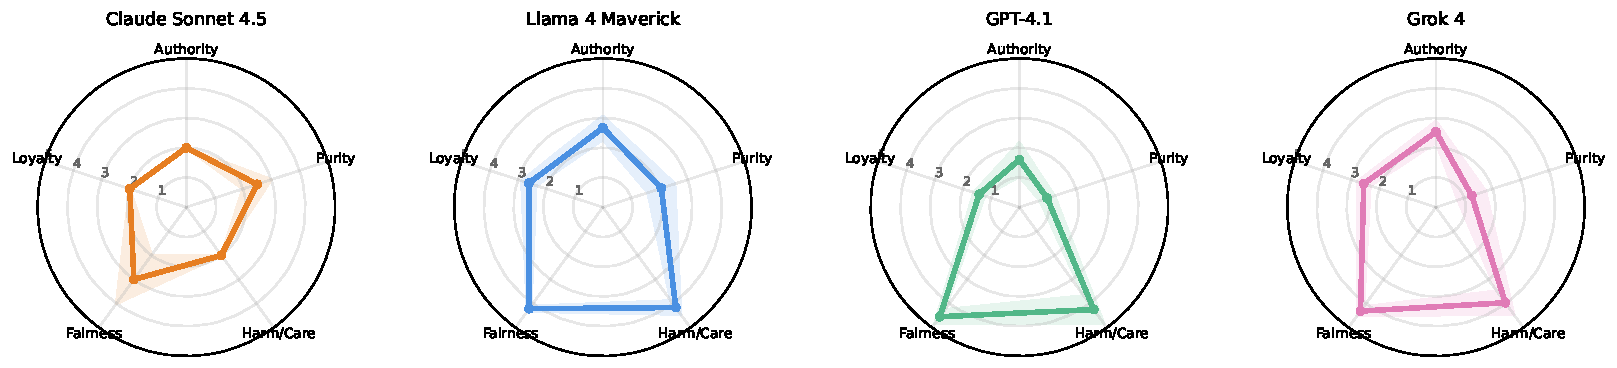
\includegraphics[width=\linewidth]{figures/moral_foundations_selected_models_radars.pdf}
  \caption{Moral foundation radar profiles for four representative no-persona responses: Claude Sonnet 4.5, DeepSeek V3.1, GPT-4o, and Grok 4. Solid lines trace mean foundation scores and shaded bands denote standard errors. The full set of model-level radar profiles appears in Appendix~\ref{app:moral-foundation-profile}; exact values are reported in Table~\ref{tab:moral_foundations_profiles}.}
  \label{fig:mfq-profiles}
\end{figure}

\begin{figure}[t!]
  \centering
  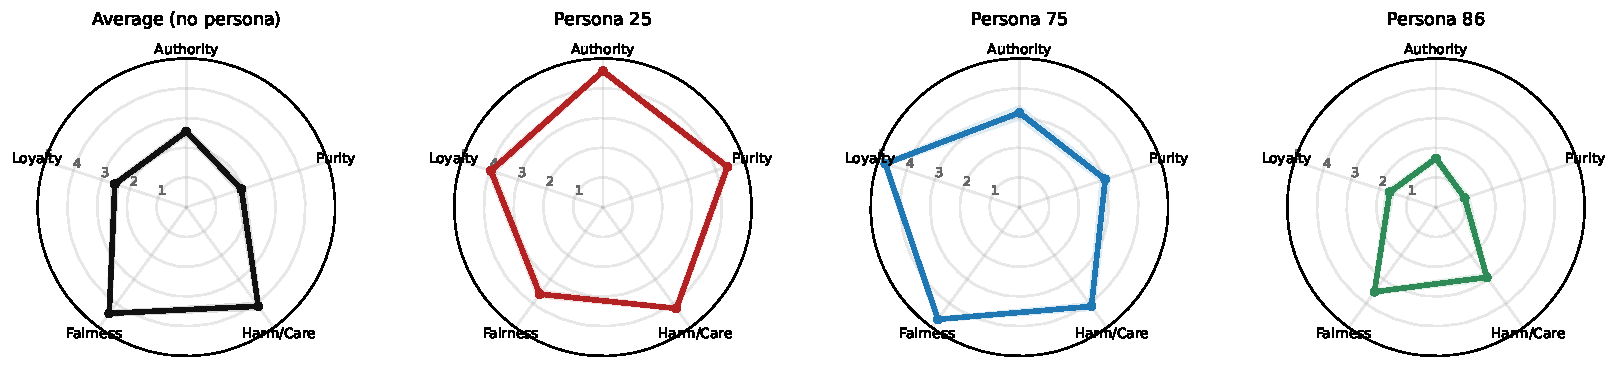
\includegraphics[width=\linewidth]{figures/moral_foundations_persona_shift_radars.pdf}
  \caption{Average moral foundation radar profile across all models with no persona-conditioning, compared with persona-averaged profiles for personas 25, 75, and 86. These personas were selected because they induce large qualitative shifts in different directions: persona 25 raises Authority/Respect and Purity/Sanctity, persona 75 raises In-group/Loyalty and Fairness/Reciprocity, and persona 86 suppresses most foundations. Solid lines trace mean foundation scores and shaded bands denote standard errors. See Table~\ref{tab:persona_moral_foundations_profiles} for exact values.}
  \label{fig:persona-mfq-profiles}
\end{figure}

Figure~\ref{fig:persona-mfq-profiles} compares the no-persona conditioning average moral profile with three persona-conditioned averages chosen to highlight large shifts in the radar. Persona 25 concentrates weight on Authority/Respect and Purity/Sanctity, persona 75 amplifies In-group/Loyalty and Fairness/Reciprocity, and persona 86 depresses all foundations, especially In-group/Loyalty, Authority/Respect, and Purity/Sanctity (see Appendix~\ref{app:personas} for the persona descriptions and Appendix~\ref{app:moral-foundation-profile} for the exact values). The full per-persona, per-model, and per-question MFQ ratings are available in our GitHub repository \cite{costa2025llmms}.

\subsection{Persona Moral Metrics}

This section formalizes the benchmark quantities and the estimators we use in practice.

Let \(\mathcal{P}\) be the set of personas and \(\mathcal{Q}\) the set of 30 scored MFQ questions. For a fixed decoding temperature \(T\), let \(Y_{pq}(T)\in\{0,\ldots,5\}\) denote the random rating produced by the model for persona \(p\) and question \(q\). We define the benchmark moments
\begin{align}
  \mu_{pq}(T) = \mathbb{E}[Y_{pq}(T)], \qquad \sigma_{pq}^2(T) = \operatorname{Var}(Y_{pq}(T)).
  \label{eq:persona-question-mean}
\end{align}
To simplify notation we suppress the explicit temperature argument below, but all quantities are defined at a fixed temperature.

\paragraph{Moral robustness} We summarize within-persona variability by averaging the standard deviations in Eq.~\eqref{eq:persona-question-mean} over personas and questions:
\begin{equation}
  \label{eq:mean-inv-robustness}
  \bar{\sigma} = \frac{1}{|\mathcal{P}||\mathcal{Q}|}\sum_{p \in \mathcal{P}}\sum_{q \in \mathcal{Q}}\sigma_{pq}
\end{equation}
and define moral robustness as
\begin{equation}
  R = \frac{1}{\bar{\sigma}}.
  \label{eq:robustness}
\end{equation}


\paragraph{Moral susceptibility} We summarize across-persona variability by computing, for each question \(q\), the variance of persona means
\begin{equation}
  \tau_q^2 = \frac{1}{|\mathcal{P}|} \sum_{p \in \mathcal{P}}(\mu_{pq} - \bar{\mu}_q)^2,
  \qquad
  \bar{\mu}_q = \frac{1}{|\mathcal{P}|} \sum_{p \in \mathcal{P}} \mu_{pq},
  \label{eq:question-dispersion}
\end{equation}
and define moral susceptibility as the average over questions
\begin{equation}
  \label{eq:overall-susceptibility}
  S = \frac{1}{|\mathcal{Q}|}\sum_{q \in \mathcal{Q}}\tau_q.
\end{equation}

Foundation-specific robustness and susceptibilities reuse Eqs.~\eqref{eq:mean-inv-robustness}--\eqref{eq:overall-susceptibility} after restricting \(\mathcal{Q}\) to the question subset \(\mathcal{Q}_f\) for foundation \(f\).

\subsection{Experimental Methodology}
\label{sec:experimental-methodology}
We use two complementary procedures to estimate the benchmark quantities above. The sampling procedure applies to all queried models and supports the main benchmark. The logit procedure is more direct, but only applies to providers that expose the next-token distribution. The common experimental setup is:

\begin{itemize}
  \item \textbf{Personas:} We evaluate $|\mathcal{P}|=100$ persona descriptions drawn from prior work \citep{ge2025scalingsyntheticdatacreation}. Full persona descriptions and the corresponding ID–description mappings are provided in Appendix~\ref{app:personas}.
  \item \textbf{Prompting:} For each persona and question, the model receives a role-playing instruction: ``You are roleplaying as the following persona:", followed by the persona description text and one of the $|\mathcal{Q}|=30$ MFQ questions.\footnote{We query one MFQ question at a time rather than the full questionnaire in a single prompt to avoid sequence- and order-dependent effects.} We instruct the models to start their response with the rating (an integer from 0 to 5), followed by their reasoning. Exact prompt templates are provided in Appendix~\ref{app:prompts}. We use decoding temperature $T=0.1$ to keep stochasticity consistent across models.
  \item \textbf{Models:} We included: Claude Haiku 4.5, Claude Sonnet 4.5, DeepSeek V3, DeepSeek V3.1, Gemini 2.5 Flash Lite, Gemini 2.5 Flash, GPT-4.1, GPT-4.1 Mini, GPT-4.1 Nano, GPT-4o, GPT-4o Mini, Grok 4, Grok 4 Fast, Llama 4 Maverick, and Llama 4 Scout.
  \item \textbf{Families:} We group the above models in the following families: Claude, DeepSeek, Gemini, GPT, Grok, and Llama.
\end{itemize}

\subsubsection{Sampling}

Sampling is the procedure we can use broadly across all benchmarked models. For the main benchmark, each persona--question pair is queried \(n=10\) times, producing parsed ratings \(y_{pqi}\in\{0,\ldots,5\}\) for repetitions \(i=1,\ldots,n\). In the first run, we constrain outputs to begin with a single integer rating from 0 to 5, and parse this leading integer. Parsing failures are recorded and we repeat each attempt, allowing responses that do not begin with the rating (see Section~\ref{sec:failures} for more details).

From these repeated samples we estimate
\begin{align}
  \hat{\mu}_{pq} = \frac{1}{n} \sum_{i=1}^{n} y_{pqi},\qquad \hat{\sigma}_{pq}^2 = \frac{1}{n-1} \sum_{i=1}^{n} \big(y_{pqi} - \hat{\mu}_{pq}\big)^2.
\end{align}
Bessel's correction applies here because it is an estimator of a broader population variance. Plugging \(\hat{\mu}_{pq}\) and \(\hat{\sigma}_{pq}\) into Eqs.~\eqref{eq:mean-inv-robustness}--\eqref{eq:overall-susceptibility} gives the repeated-query estimates of \(R\) and \(S\). We estimate the uncertainty of \(S\) and \(R\) by bootstrap resampling over personas. For each model, this sampling pipeline requires $|\mathcal{Q}|\times|\mathcal{P}|\times n =30\times 100\times 10=30,000$ requests.

\subsubsection{Logit}
\label{sec:logit}

For providers that expose next-token logits, we implemented a more direct alternative. Given that the prompt asks the model to begin its response with a rating from 0 to 5 (see Appendix~\ref{app:prompts}), the logit associated with that next-token gives a direct estimate of the desired probability distribution. Let \(z_n\) denote the next-token logit assigned to digit \(n\in\{0,\ldots,5\}\). We define the induced digit probabilities at temperature $T$ as
\begin{align}
  p_n(T) = \frac{\exp(z_n/T)}{\sum_{m=0}^5 \exp(z_m/T)},
  \label{eq:probabilities}
\end{align}
and compute the corresponding mean score and variance as
\begin{align}
  \mu_{pq}(T) = \sum_{n=0}^5 n p_n(T), \quad \sigma_{pq}^2 = \sum_{n=0}^5 (n-\mu_{pq}(T))^2 p_n(T).
\end{align}
This logit-based procedure has two practical benefits: it almost completely eliminates parsing failures, and it removes the need to query the same persona--question pair multiple times. 

In practice, the APIs we used return next-token log-probabilities rather than raw logits, but this gives the same probability distribution because the additive constant factors out in Eq. \eqref{eq:probabilities}. The main approximation comes from the OpenAI APIs, which only return a top-20 next-token list. When one of the six digits is absent from that list, we assign it the smallest returned log-probability. This conservative rule mildly overestimates the probability mass of omitted digits and therefore slightly inflates uncertainty; Appendix~\ref{sec:logit-uncertainty} quantifies the size of this effect.

\subsection{Temperature Dependence}
\label{sec:rating_estimation}

For the subset of models where we collected next-token logits, we can additionally study how both metrics change as a function of temperature by dialing it in Eq.~\eqref{eq:probabilities}. Figure~\ref{fig:logprob-temperature} shows this construction for the OpenAI models (GPT-4o, GPT-4o Mini, GPT-4.1, GPT-4.1 Mini, and GPT-4.1 Nano), with shaded bands reporting persona-bootstrap uncertainty. As a cross-check, we additionally collected \(n=50\) repeated samples at \(T \in \{0.4, 0.8, 1.2\}\) for the smallest variants of each family; the resulting points are overlaid on the figure and are in good agreement with the logit-derived curves. Moral robustness decreases rapidly as temperature increases ($R \to \infty$ as $T \to 0$, since $\bar{\sigma} \to 0$ in the deterministic limit), while moral susceptibility changes more moderately. Robustness curve separation between models grows as temperature decreases, and the model-specific curves do not cross within the temperature range studied. These observations support reporting the benchmark at $T=0.1$.

\begin{figure}[t!]
  \centering
  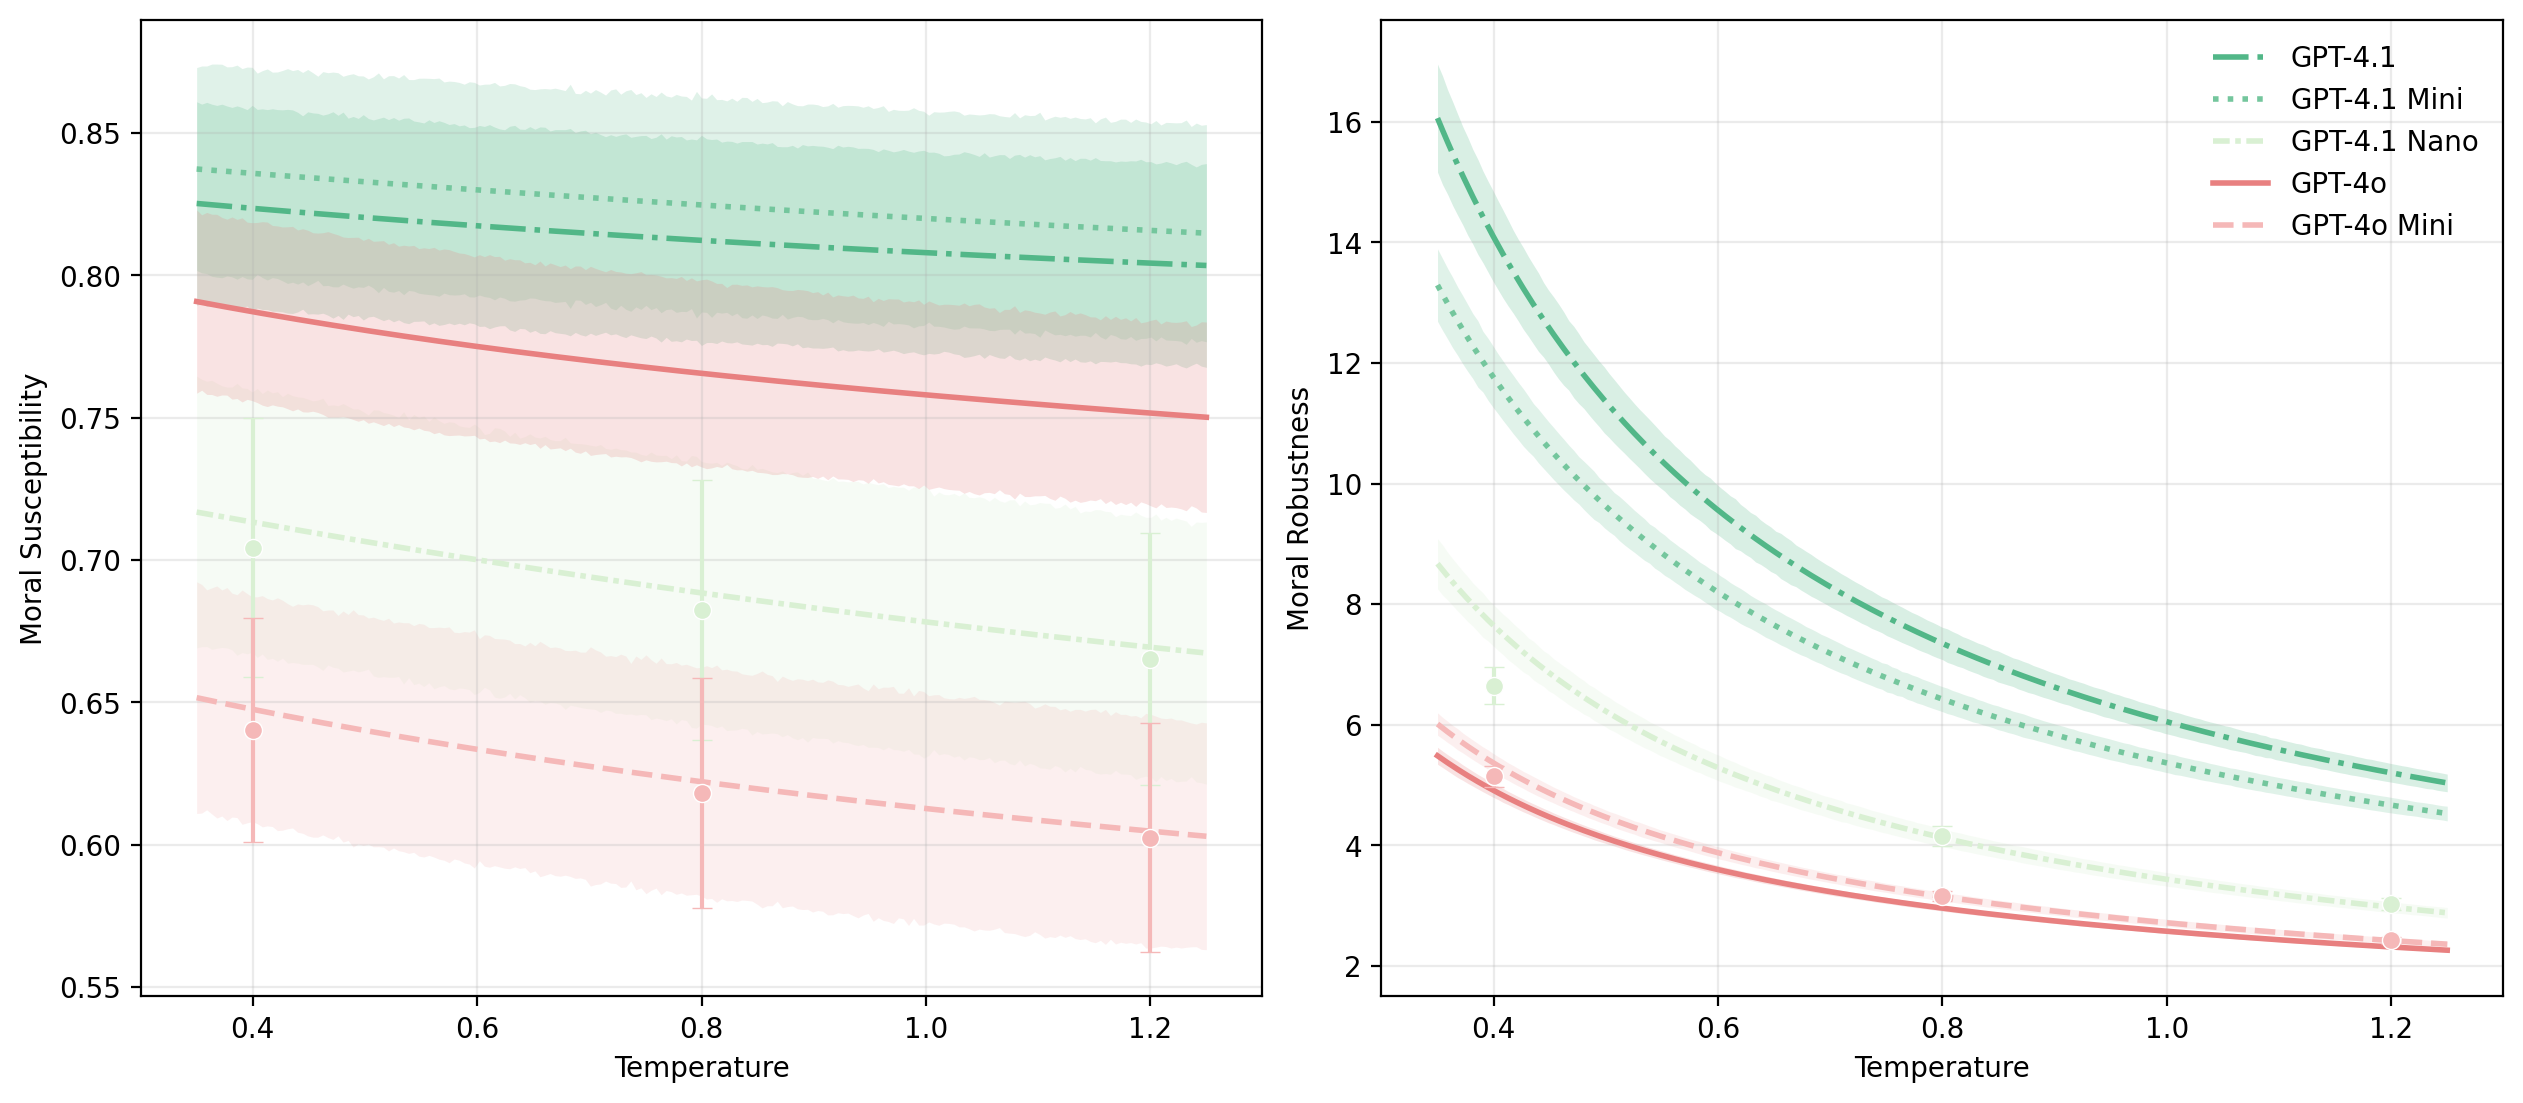
\includegraphics[width=\linewidth]{figures/temperature_metrics_from_logprobs_combined.png}
  \caption{Temperature dependence of moral robustness and moral susceptibility derived from next-token logits, shaded bands report persona-bootstrap uncertainty (see Section~\ref{sec:logit} for reference). The sampled points come from direct temperature sweeps with \(n=50\) repetitions per persona--question pair, with error bars coming from both persona and run bootstrap.}
  
  \label{fig:logprob-temperature} 
\end{figure}



\section{Results}

\subsection{Model Rankings at \texorpdfstring{$T=0.1$}{T=0.1}}
\label{sec:benchmark-ranking}

Figure~\ref{fig:benchmark-bars} shows robustness and susceptibility separately as one-dimensional rankings at \(T=0.1\). The two metrics differ markedly in their across-model spread: robustness has a coefficient of variation of about 152\%, with the most robust model roughly 33 times more robust than the least, whereas susceptibility has a coefficient of variation of only about 13\%, with the most susceptible model just 1.6 times more susceptible than the least. The robustness panel makes the family structure immediately visible: the Claude models lead by a substantial margin, followed by Gemini and GPT-4 variants, while Grok, DeepSeek, and Llama remain less robust. The susceptibility panel has a much tighter spread, with Gemini 2.5 Flash and Grok 4 Fast among the most susceptible models and Llama 4 Scout among the least susceptible. This view is useful for direct model ranking, while the joint geometry of the two metrics is easier to inspect in the scatter map of Figure~\ref{fig:overall-rs-scatter}.

\begin{figure*}[t!]
  \centering
  \begin{minipage}[t]{0.49\textwidth}
    \centering
    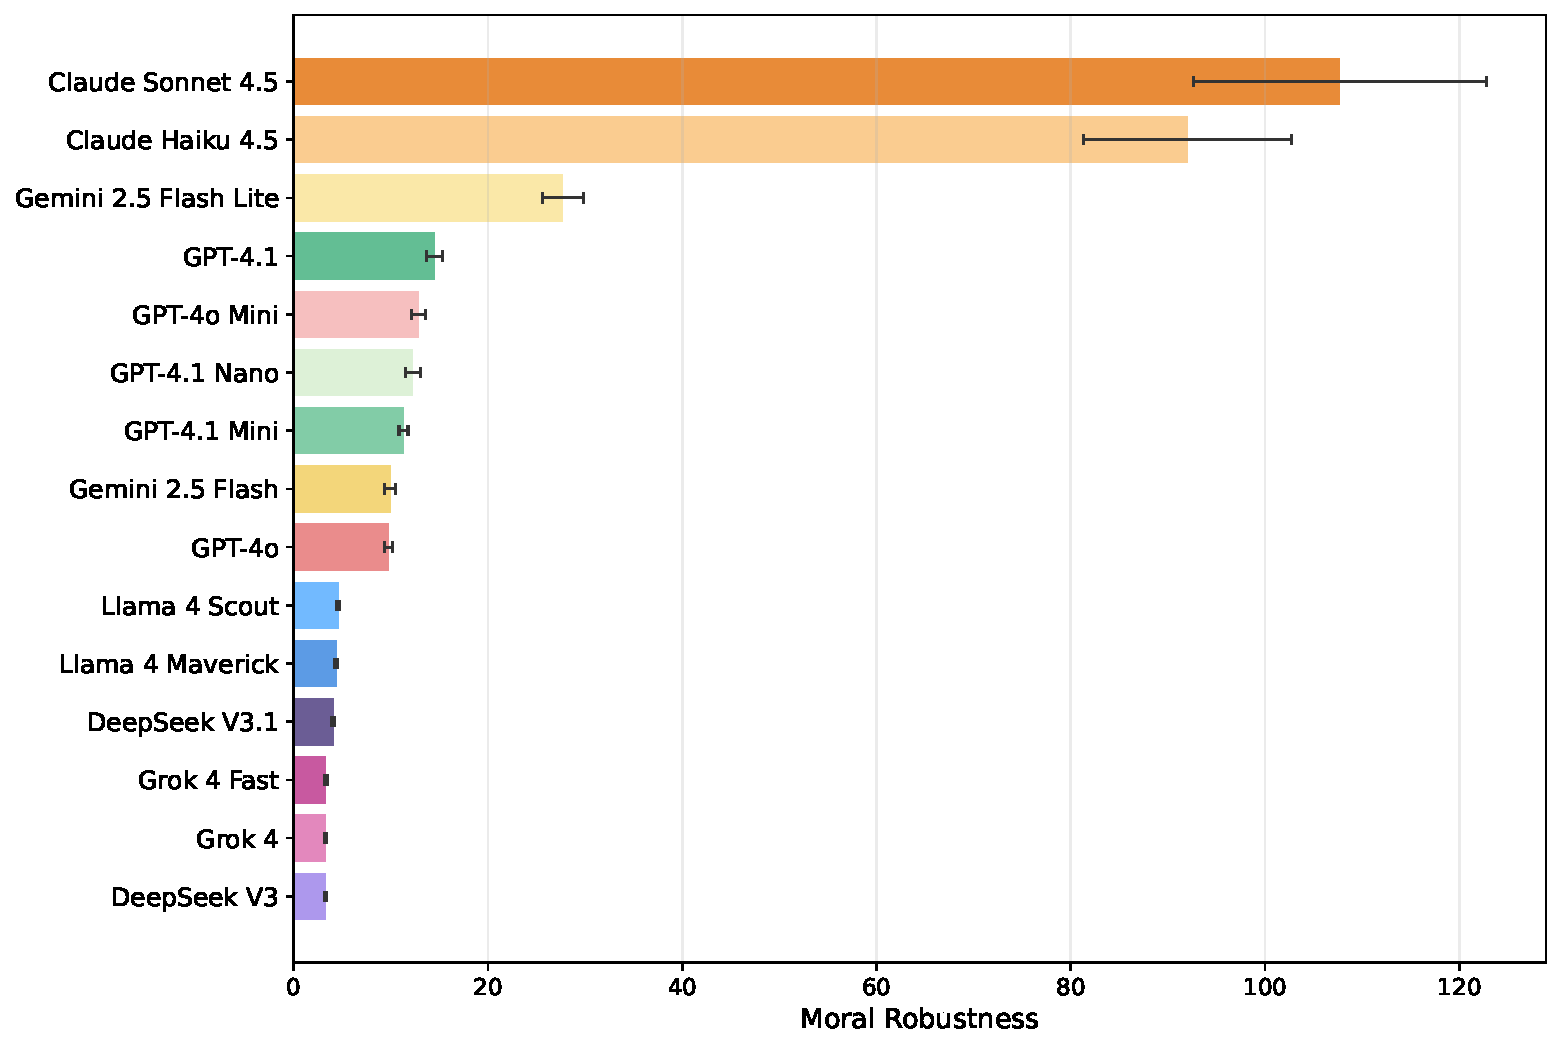
\includegraphics[width=\linewidth]{robustness_temp01.pdf}
  \end{minipage}\hfill
  \begin{minipage}[t]{0.49\textwidth}
    \centering
    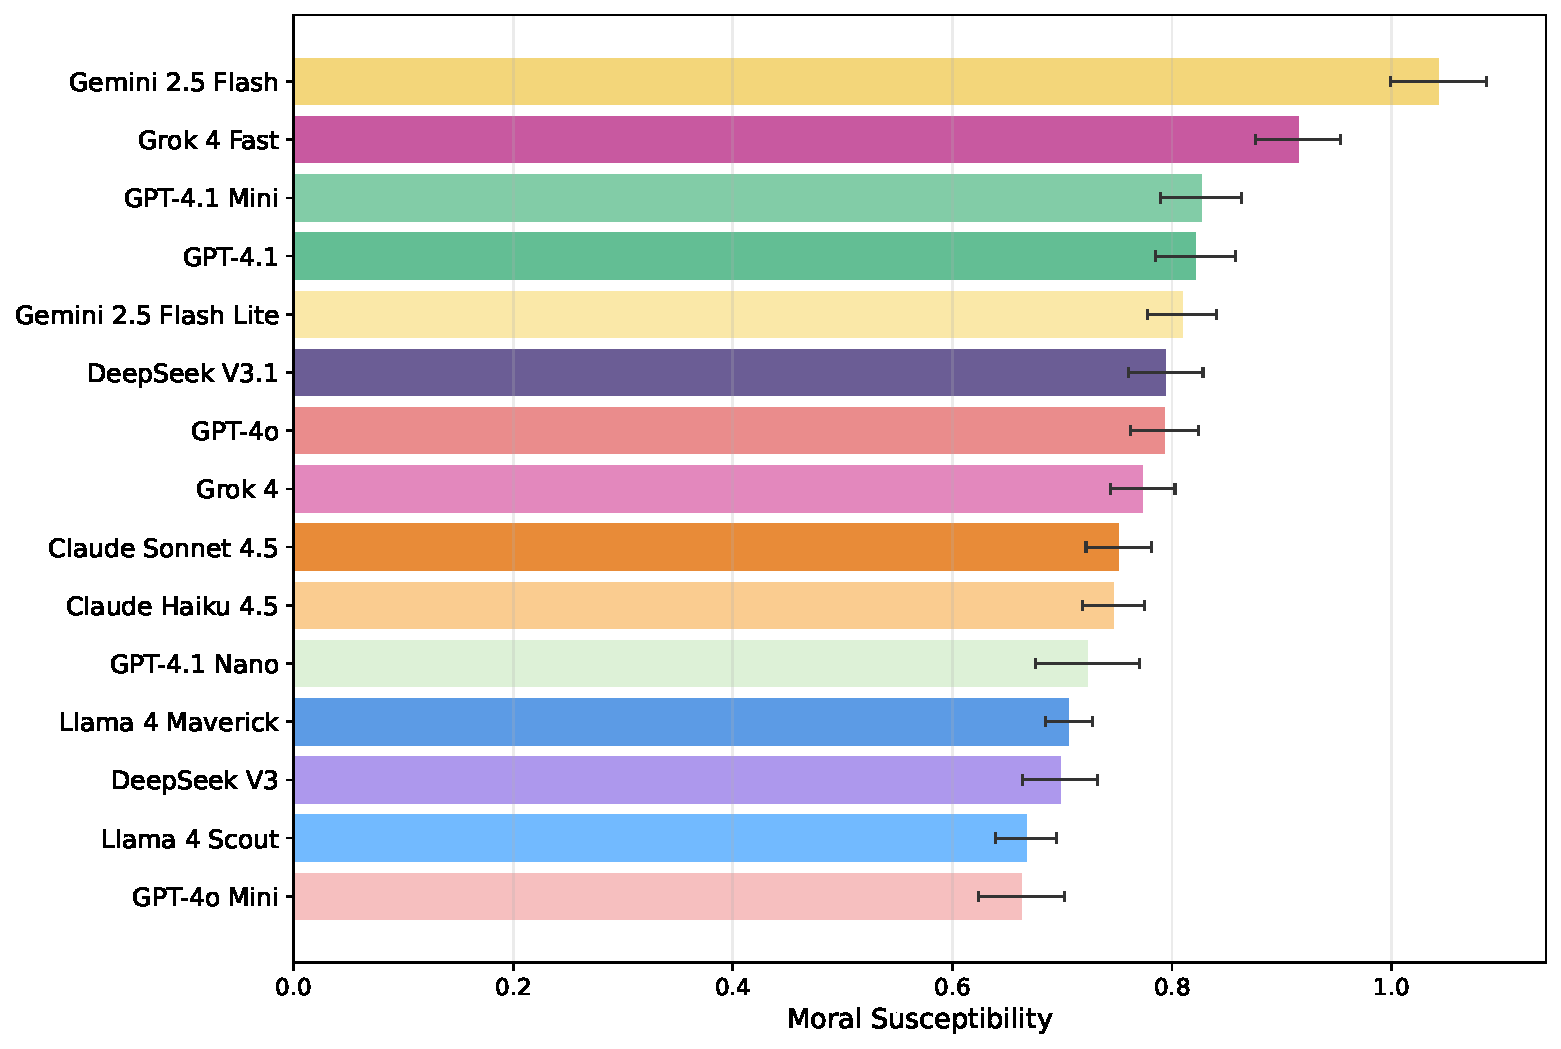
\includegraphics[width=\linewidth]{susceptibility_temp01.pdf}
  \end{minipage}
  \caption{Model rankings at \(T=0.1\). Left: moral robustness. Right: moral susceptibility. Error bars combine persona-bootstrap and rerun-bootstrap uncertainty from the sampled metrics.}
  \label{fig:benchmark-bars}
\end{figure*}


\subsection{Overall Robustness--Susceptibility Map}
\label{sec:overall-rs-map}

Figure~\ref{fig:overall-rs-scatter} complements the benchmark rankings by displaying the joint distribution of the overall robustness and susceptibility indices for each model. We use a logarithmic robustness axis because \(R\) spans more than one order of magnitude. The Claude models occupy the far-right portion of the plot, indicating substantially higher robustness than the rest of the benchmark. DeepSeek, Grok, and Llama remain on the low-robustness side, while GPT-4 and Gemini models lie between these extremes. Along the susceptibility axis the spread is much narrower: Gemini 2.5 Flash is the most susceptible overall, Grok 4 Fast is also highly susceptible despite very low robustness, and Llama 4 Scout is the least susceptible. The overall cloud does not exhibit a strong monotonic relationship between \(R\) and \(S\); instead, model families form distinct clusters. A Pearson correlation between \(\log R\) and \(S\) across the 15 models confirms this: \(r = -0.03\) (\(p = 0.91\)), indicating that robustness and susceptibility are essentially orthogonal dimensions at the model level.

\begin{figure}[t!]
  \centering
  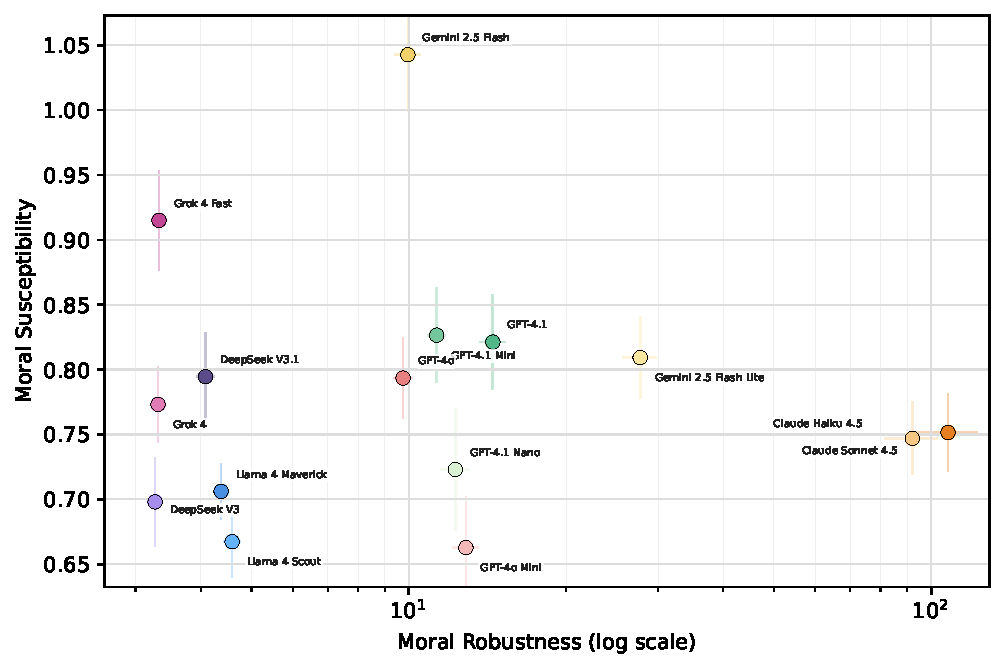
\includegraphics[width=\linewidth]{figures/moral_metrics_overall_scatter.pdf}
  \caption{Overall robustness--susceptibility map across models. The horizontal axis uses a logarithmic scale to accommodate the wide range of robustness values. Each point is annotated with a short model label and error bars denote standard errors.}
  \label{fig:overall-rs-scatter}
\end{figure}

\subsection{Family Structure and Size Trends}
\label{sec:family-size-trends}

The clustering visible in Figure~\ref{fig:overall-rs-scatter} can be quantified directly. Robustness varies widely across the 15 benchmarked models, with a coefficient of variation of about 152\% and the most robust model (Claude Sonnet 4.5, $R\approx 108$) roughly 33 times more robust than the least (DeepSeek V3, Grok 4, and Grok 4 Fast, all near $R\approx 3.3$). A one-way permutation ANOVA on \(\log R\) grouped by provider family (Claude, DeepSeek, Gemini, GPT, Grok, and Llama) yields \(\eta^2 = 0.963\) with permutation \(p < 2 \times 10^{-5}\), indicating that family membership explains nearly all of this variation. In this ordering, the Claude models sit far above the rest, Gemini and GPT occupy an intermediate band, and Llama, DeepSeek, and Grok cluster at the low-robustness end. The combination of large across-model variance, near-complete family-level explanation, and absent size effect is evidence that robustness is primarily determined by post-training, reflecting alignment-stage choices rather than scale.

Susceptibility behaves differently. Across the same 15 models, $S$ has a coefficient of variation of only about 13\%, and the most susceptible model (Gemini 2.5 Flash, $S\approx 1.04$) is only 1.6 times more susceptible than the least (GPT-4o Mini, $S\approx 0.66$). A matching permutation ANOVA on \(S\) grouped by the same six families yields \(\eta^2 = 0.539\) with permutation \(p = 0.137\), so the family structure in susceptibility is weaker and does not reach conventional significance at this sample size. The size trend is also weak. Because parameter counts are not publicly available for several closed-source models, we operationalize size with an ordinal within-series rank: rank 0 for the smallest variant in each series, incremented for each next-larger variant. The seven series in our benchmark are Claude 4.5 (Haiku, Sonnet), DeepSeek (V3, V3.1, a version progression), Gemini 2.5 Flash (Lite, full), GPT-4o (Mini, full), GPT-4.1 (Nano, Mini, full), Grok 4 (Fast, full), and Llama 4 (Scout, Maverick). Regressing $S$ on the within-series rank with a separate intercept per series gives a positive slope of \(\beta_S = 0.056 \pm 0.035\) susceptibility units per rank step (\(\Delta R^2 = 0.269\), permutation \(p = 0.150\)), consistent with a mild tendency for larger variants to be more susceptible but admitting model-specific exceptions. Together, the low across-model variance, the absent family structure, and the mild size dependence point to susceptibility being primarily determined by pre-training, reflecting statistical regularities of the shared text corpora and objectives behind modern LLMs rather than alignment-stage choices.

\subsection{Foundation-Level Decomposition}
\label{sec:foundation-rs-map}

Figure~\ref{fig:foundation-rs-radars} decomposes each model's foundation-level behavior into two normalized profiles. The solid curve shows the susceptibility shares \(S_f / S\), while the dashed curve shows the corresponding inverse-robustness shares \(\overline{\sigma}_f / \overline{\sigma}\). Because both profiles are normalized to sum to one, the radar shape isolates where each model concentrates its persona sensitivity and within-persona inverse robustness, while the overall scale remains visible in Figure~\ref{fig:overall-rs-scatter}. Several family-level regularities are apparent: Gemini and DeepSeek variants allocate relatively large susceptibility mass to Authority/Respect and Purity/Sanctity, Claude models concentrate more of their inverse robustness in Authority/Respect and Loyalty while remaining globally robust, and Llama and Grok variants show flatter inverse-robustness profiles with sharper susceptibility peaks. Exact foundation-level \(R_f\) and \(S_f\) values are reported in Appendix~\ref{app:metric-values}.

To test whether robustness and susceptibility are coupled at the foundation level, we compute Pearson correlations between \(\log R_f\) and \(S_f\) across the 15 models separately for each foundation. Four of the five foundations show no significant association (Harm/Care: \(r=0.13\), \(p=0.63\); Fairness/Reciprocity: \(r=0.22\), \(p=0.44\); In-group/Loyalty: \(r=0.03\), \(p=0.91\); Authority/Respect: \(r=-0.26\), \(p=0.36\)). Purity/Sanctity is the exception: \(r=-0.49\) (\(p=0.07\)), suggesting a moderate negative association in which more robust models also tend to be less susceptible specifically on this foundation.

\begin{figure*}[t!]
  \centering
  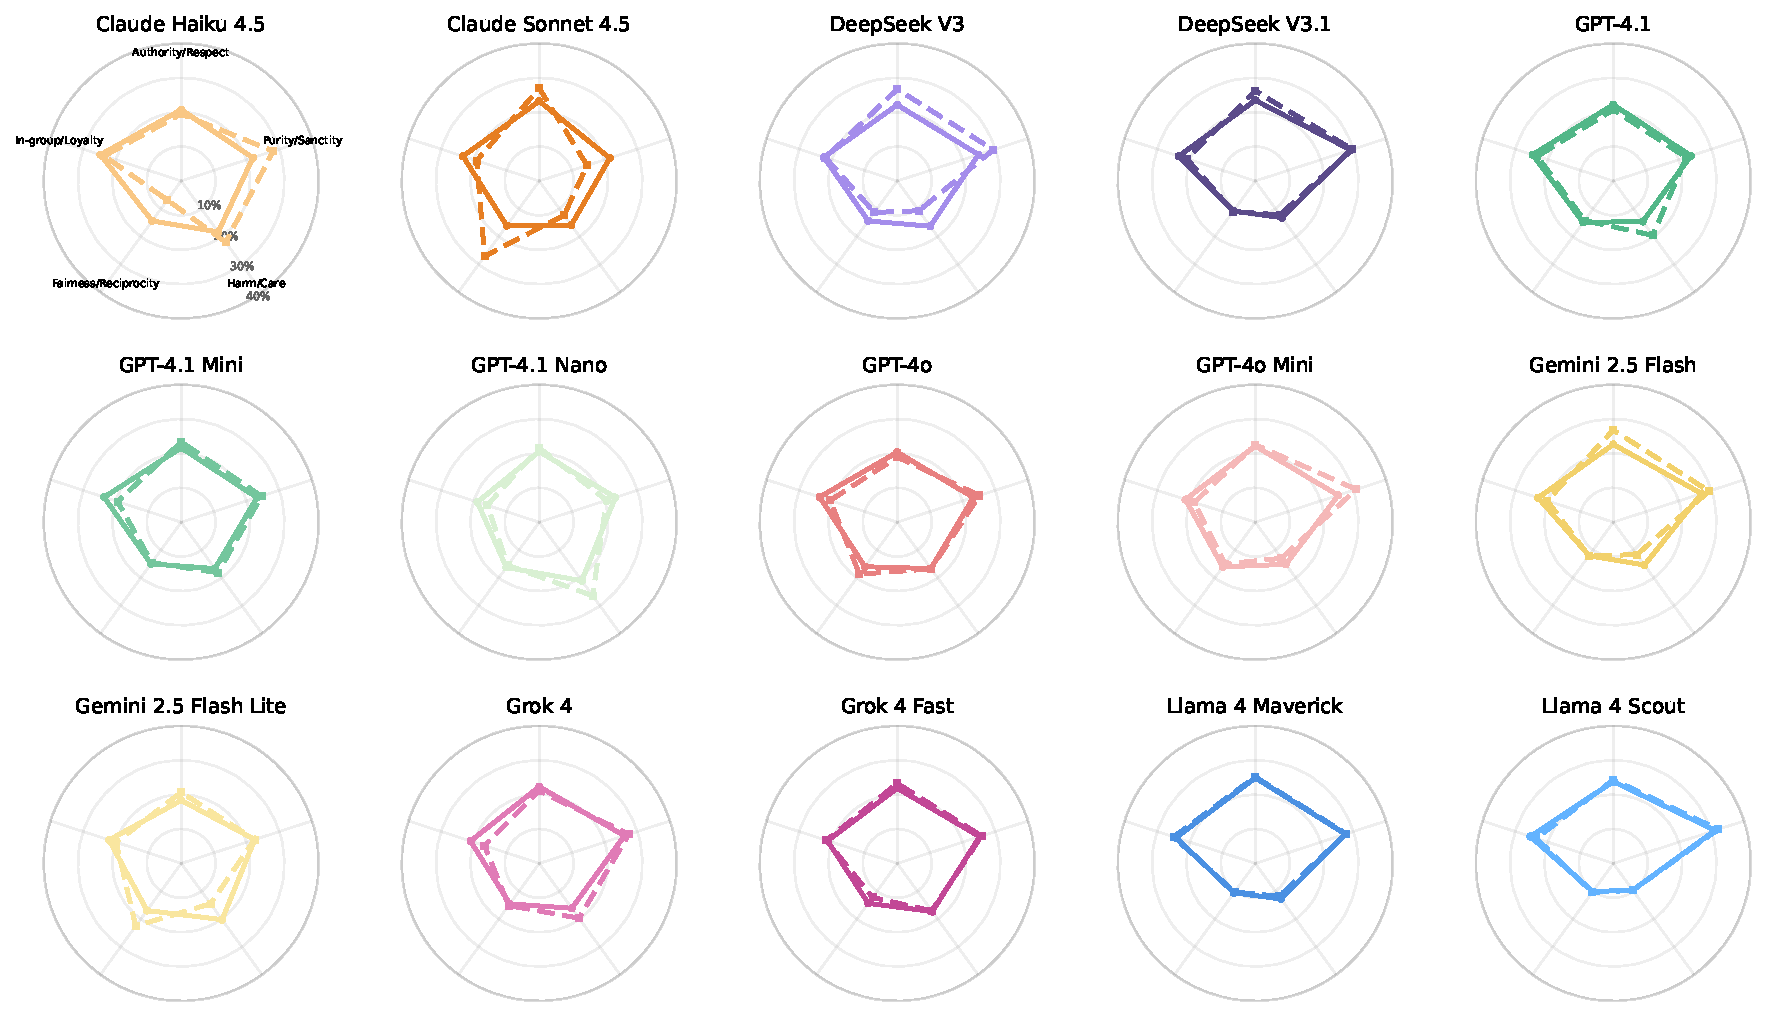
\includegraphics[width=\linewidth]{figures/moral_metrics_foundation_decomposition_radars.pdf}
  \caption{Foundation-level decomposition of susceptibility and inverse robustness for all benchmarked models. For each model, the solid curve shows the susceptibility shares \(S_f / S\), while the dashed curve shows the corresponding inverse robustness shares \(\overline{\sigma}_f / \overline{\sigma}\). All curves use the same radial range from 0 to 40\%, with foundations ordered as in the first radar.}
  \label{fig:foundation-rs-radars}
\end{figure*}

\FloatBarrier

\section{Discussion and Future Directions}
\label{sec:discussion}

\paragraph{Post-training as the driver of moral robustness.}
Robustness varies widely across the benchmark (coefficient of variation $\approx 152\%$), and the near-perfect family-level explanation of this variance ($\eta^2 = 0.963$) is difficult to attribute to scale, since model size shows no systematic effect while provider families remain sharply separated. This points to post-training, including alignment fine-tuning, RLHF, and constitutional procedures, as a plausible primary determinant of moral robustness.

\paragraph{Pre-training as the driver of moral susceptibility.}
Susceptibility shows the opposite pattern. It varies little across the benchmark (coefficient of variation $\approx 13\%$), shows no family-level structure, and depends only mildly on size within families. The combination of low across-model variance, absent family effects, and weak size dependence is naturally explained by pre-training, including the shared text corpora and objectives that underlie modern LLMs, rather than by alignment-stage choices. Under this view, persona susceptibility reflects common statistical regularities in how text describes morally relevant traits, regularities that current alignment procedures leave largely intact.

\paragraph{Constitutional AI and persona competence.}
The Claude family's robustness advantage invites a more specific hypothesis. Constitutional AI \citep{bai2022constitutional} involves iterative self-critique against a set of principles, repeatedly exercising the model's ability to reason about how agents with different values would respond to moral scenarios. We conjecture that this training produces a more calibrated internal representation of each persona's moral reasoning, rather than mere resistance to persona conditioning. Consistent with this, Claude's susceptibility is not the lowest in the benchmark: it shifts meaningfully across personas, but does so with low within-persona variance.

\paragraph{Future directions.}
A natural extension is to apply the benchmark to other moral psychology instruments and richer persona sets, to test how far the family-level robustness structure generalizes. Because $R$ and $S$ are derived from a fixed instrument and persona set, the $(R, S)$ plane can also be used to track and compare training interventions: each intervention leaves a signature in the plane, and distinct signatures correspond to qualitatively different effects \citep{costa2026personacollapse}.

\section{Conclusion}
We introduced a benchmark for measuring how persona role-play changes moral judgments in large language models using the Moral Foundations Questionnaire, separating within-persona variability (moral robustness) from across-persona variability (moral susceptibility) and estimating both quantities through repeated sampling, with a complementary logit-based procedure when next-token distributions are available. Across 15 models and six families, moral robustness varies by more than an order of magnitude (coefficient of variation $\approx 152\%$), shows a strong family structure with Claude models substantially more robust than the rest, and is unaffected by size, suggesting that it is primarily determined by post-training. Moral susceptibility, in contrast, varies over a much narrower range (coefficient of variation $\approx 13\%$), shows no family dependence, and exhibits only a mild within-family size trend, suggesting that it is primarily determined by pre-training. At the model level, robustness and susceptibility are largely orthogonal, and the foundation-level decomposition shows that families concentrate persona sensitivity and inverse robustness in different moral foundations. Overall, persona conditioning reveals structured, model-dependent moral shifts rather than a single generic effect, providing a quantitative basis for future work on social reasoning and alignment evaluation under persona role-play.


%\section*{Acknowledgments}
%
%We gratefully acknowledge the financial support of the TELUS Digital Research Hub.
\section*{Ethics Statement}

This paper presents work whose goal is to advance the understanding of moral behavior in large language models by systematically analyzing how moral judgments change under persona role-play. By introducing a benchmark grounded in moral psychology, this work may contribute to improved evaluation and design of more reliable and value-aligned AI systems. At the same time, insights into moral susceptibility could potentially be misused to deliberately influence or manipulate model outputs in sensitive contexts. We view this research as primarily foundational and methodological, and we do not anticipate significant negative societal consequences beyond those already well established for research on model alignment and controllability.

\section*{Reproducibility Statement}

All code, prompts, and processed results needed to reproduce our experiments are publicly available in our GitHub repository \cite{costa2025llmms}. The exact prompt formats used to query the models are detailed in Appendix~\ref{app:prompts}. The full list of personas is provided in Appendix~\ref{app:personas}. Raw model outputs, persona-level MFQ response matrices and logit vectors are also included.

\bibliographystyle{colm2026_conference}
\bibliography{references}


\appendix

\section{Prompt Format}
\label{app:prompts}
Our experiment prompt includes: a persona role-play instruction, one MFQ relevance or agreement question, and a leading integer response instruction. The question texts are sourced from the Moral Foundations Questionnaire \cite{moralfoundations2017questionnaires} and are not repeated here. Below we show the exact prompt formats used.

\textbf{Persona role-play instruction.}
\begin{quote}
\ttfamily\scriptsize
You are roleplaying as the following persona: 
<DESCRIPTION>

Please answer the following question.
\end{quote}

\textbf{Relevance question template.}
\begin{quote}
\ttfamily\scriptsize
When deciding whether something is right or wrong, how relevant is the following consideration to your thinking: <CONSIDERATION>. Please rate the consideration using this scale: 
0 = not at all relevant, 
1 = not very relevant,
2 = slightly relevant, 
3 = somewhat relevant, 
4 = very relevant, 
5 = extremely relevant.
\end{quote}

\textbf{Agreement question template.}
\begin{quote}
\ttfamily\scriptsize
Please indicate your level of agreement with the following statement: <STATEMENT>. Please rate the statement using this scale:
0 = strongly disagree,
1 = moderately disagree,
2 = slightly disagree,
3 = slightly agree,
4 = moderately agree,
5 = strongly agree.
\end{quote}

\textbf{Leading integer response instruction.}
\begin{quote}
\ttfamily\scriptsize
Your response should start with an integer from 0 to 5, followed by your reasoning.
\end{quote}

The three bracketed words iterated respectively over: persona text descriptions (see Appendix~\ref{app:personas}); the 15 relevance MFQ questions, and the 15 agreement MFQ questions.

\section{Moral Foundation Profile}
\label{app:moral-foundation-profile}
This appendix provides the numerical MFQ foundation profiles that correspond to Figures~\ref{fig:mfq-profiles} and~\ref{fig:persona-mfq-profiles}. Table~\ref{tab:moral_foundations_profiles} reports the no-persona scores for each model, while Table~\ref{tab:persona_moral_foundations_profiles} lists the average scores for the three personas highlighted in the main text. Each entry is the mean rating with its associated standard error.

\begin{table}[t!]
  \centering
  \caption{MFQ foundation profiles for no-persona responses. Values are mean ratings with standard errors computed across repeated questionnaire runs.}
  \label{tab:moral_foundations_profiles}
  \resizebox{\linewidth}{!}{% Auto-generated by analysis/generate_relevance_profile_tables.py
\begin{tabular}{lccccc}
  \toprule
  Model & Harm/Care & Fairness/Reciprocity & In-group/Loyalty & Authority/Respect & Purity/Sanctity \\
  \midrule
  Claude Haiku 4.5 & $3.50\pm0.50$ & $3.83\pm0.17$ & $1.83\pm0.17$ & $2.17\pm0.17$ & $2.00\pm0.26$ \\
  Claude Sonnet 4.5 & $2.00\pm0.00$ & $3.00\pm1.00$ & $2.00\pm0.00$ & $2.00\pm0.00$ & $2.50\pm0.50$ \\
  DeepSeek V3 & $4.57\pm0.43$ & $4.72\pm0.28$ & $2.95\pm0.27$ & $3.20\pm0.37$ & $2.55\pm0.21$ \\
  DeepSeek V3.1 & $4.50\pm0.50$ & $4.82\pm0.18$ & $2.92\pm0.43$ & $2.48\pm0.61$ & $1.35\pm0.52$ \\
  Gemini 2.5 Flash & $4.35\pm0.65$ & $4.97\pm0.03$ & $2.82\pm0.31$ & $2.90\pm0.42$ & $1.97\pm0.69$ \\
  Gemini 2.5 Flash Lite & $4.50\pm0.22$ & $4.33\pm0.33$ & $1.82\pm0.87$ & $2.33\pm0.84$ & $0.83\pm0.54$ \\
  GPT-4.1 & $4.25\pm0.57$ & $4.55\pm0.30$ & $1.42\pm0.19$ & $1.60\pm0.56$ & $0.98\pm0.26$ \\
  GPT-4.1 Mini & $4.50\pm0.34$ & $4.72\pm0.18$ & $2.57\pm0.33$ & $2.32\pm0.56$ & $1.37\pm0.50$ \\
  GPT-4.1 Nano & $3.85\pm0.17$ & $3.95\pm0.05$ & $3.65\pm0.21$ & $3.13\pm0.31$ & $3.52\pm0.22$ \\
  GPT-4o & $4.42\pm0.42$ & $4.28\pm0.32$ & $2.26\pm0.37$ & $2.35\pm0.50$ & $1.83\pm0.48$ \\
  GPT-4o Mini & $5.00\pm0.00$ & $4.73\pm0.18$ & $2.98\pm0.02$ & $3.18\pm0.32$ & $3.32\pm0.17$ \\
  Grok 4 & $3.97\pm0.49$ & $4.32\pm0.18$ & $2.55\pm0.23$ & $2.53\pm0.35$ & $1.27\pm0.49$ \\
  Grok 4 Fast & $4.02\pm0.79$ & $4.88\pm0.12$ & $2.17\pm0.29$ & $2.40\pm0.49$ & $1.37\pm0.62$ \\
  Llama 4 Maverick & $4.17\pm0.28$ & $4.22\pm0.11$ & $2.62\pm0.25$ & $2.67\pm0.39$ & $2.07\pm0.48$ \\
  Llama 4 Scout & $4.12\pm0.82$ & $4.83\pm0.17$ & $3.37\pm0.50$ & $2.93\pm0.50$ & $2.28\pm0.77$ \\
  Average (no persona) & $4.11\pm0.12$ & $4.41\pm0.08$ & $2.53\pm0.09$ & $2.55\pm0.12$ & $1.95\pm0.12$ \\
  \bottomrule
\end{tabular}
}
\end{table}

\begin{table}[t!]
  \centering
  \caption{MFQ foundation profiles for personas 25, 75, and 86 used in Figure~\ref{fig:persona-mfq-profiles}, averaged across models. Values are mean ratings with standard errors computed over models and repeated questionnaire runs.}
  \label{tab:persona_moral_foundations_profiles}
  \resizebox{\linewidth}{!}{% Auto-generated by analysis/generate_relevance_profile_tables.py
\begin{tabular}{lccccc}
  \toprule
  Persona & Harm/Care & Fairness/Reciprocity & In-group/Loyalty & Authority/Respect & Purity/Sanctity \\
  \midrule
  25 & $4.20\pm0.07$ & $3.61\pm0.11$ & $3.96\pm0.11$ & $4.58\pm0.08$ & $4.40\pm0.10$ \\
  75 & $4.12\pm0.12$ & $4.66\pm0.07$ & $4.74\pm0.08$ & $3.18\pm0.21$ & $3.03\pm0.15$ \\
  86 & $2.91\pm0.12$ & $3.51\pm0.08$ & $1.63\pm0.12$ & $1.64\pm0.11$ & $1.02\pm0.13$ \\
  \bottomrule
\end{tabular}
}
\end{table}

Figure~\ref{fig:appendix-model-radars} provides one no-persona radar profile per model. This appendix figure expands the abbreviated selection shown in Figure~\ref{fig:mfq-profiles}.

\begin{figure*}[p!]
  \centering
  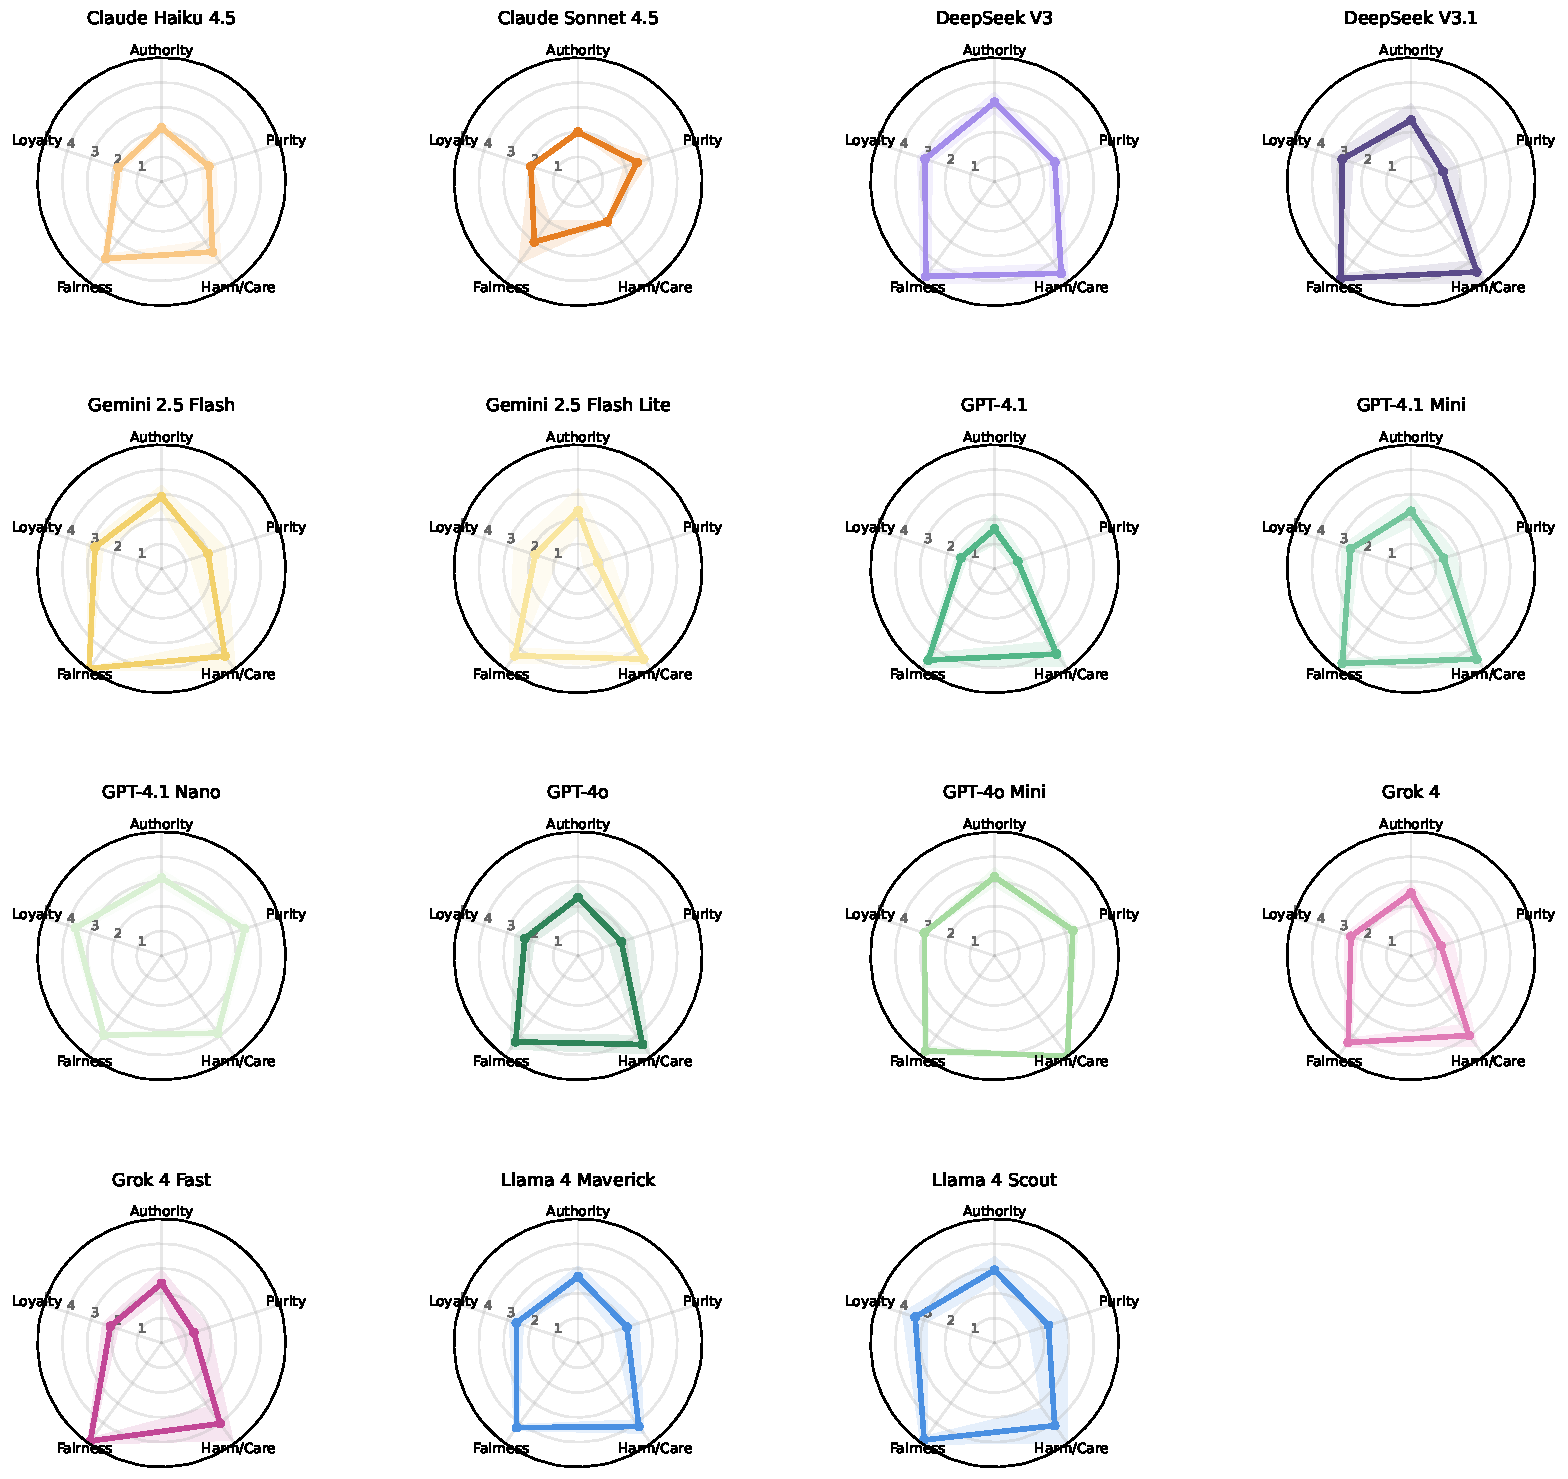
\includegraphics[width=\linewidth]{figures/moral_foundations_all_models_radars.pdf}
  \caption{Individual no-persona moral foundation radar profiles for all benchmarked models. Solid lines trace mean foundation scores and shaded bands denote standard errors.}
  \label{fig:appendix-model-radars}
\end{figure*}

\section{Robustness and Susceptibility Exact Values}
\label{app:metric-values}

Table~\ref{tab:metric_values_overall} reports the exact overall robustness and susceptibility values underlying Figure~\ref{fig:overall-rs-scatter}. Tables~\ref{tab:metric_values_harm_care}--\ref{tab:metric_values_purity_sanctity} report the corresponding foundation-specific values underlying Figure~\ref{fig:foundation-rs-radars}.

\begin{table}[t!]
  \centering
  \caption{Exact overall robustness and susceptibility values by model. Values are mean $\pm$ standard error.}
  \label{tab:metric_values_overall}
  \small
  \begin{tabular}{lcc}
    \toprule
    Model & $R$ & $S$ \\
    \midrule
    Claude Haiku 4.5 & $92.04 \pm 10.72$ & $0.747 \pm 0.028$ \\
    Claude Sonnet 4.5 & $107.70 \pm 15.08$ & $0.751 \pm 0.030$ \\
    DeepSeek V3 & $3.27 \pm 0.07$ & $0.698 \pm 0.034$ \\
    DeepSeek V3.1 & $4.08 \pm 0.16$ & $0.794 \pm 0.034$ \\
    GPT-4.1 & $14.48 \pm 0.83$ & $0.821 \pm 0.037$ \\
    GPT-4.1 Mini & $11.31 \pm 0.46$ & $0.827 \pm 0.037$ \\
    GPT-4.1 Nano & $12.28 \pm 0.77$ & $0.723 \pm 0.047$ \\
    GPT-4o & $9.75 \pm 0.42$ & $0.793 \pm 0.031$ \\
    GPT-4o Mini & $12.86 \pm 0.73$ & $0.663 \pm 0.039$ \\
    Gemini 2.5 Flash & $9.96 \pm 0.56$ & $1.043 \pm 0.044$ \\
    Gemini 2.5 Flash Lite & $27.73 \pm 2.10$ & $0.809 \pm 0.032$ \\
    Grok 4 & $3.31 \pm 0.09$ & $0.773 \pm 0.029$ \\
    Grok 4 Fast & $3.33 \pm 0.11$ & $0.915 \pm 0.039$ \\
    Llama 4 Maverick & $4.37 \pm 0.14$ & $0.706 \pm 0.022$ \\
    Llama 4 Scout & $4.59 \pm 0.16$ & $0.667 \pm 0.028$ \\
    \bottomrule
  \end{tabular}
\end{table}


\begin{table*}[p!]
  \centering
  \caption{Exact robustness and susceptibility values for Harm/Care. Values are mean $\pm$ standard error.}
  \label{tab:metric_values_harm_care}
  \small
  \begin{tabular}{lcc}
    \toprule
    Model & $R$ & $S$ \\
    \midrule
    Claude Haiku 4.5 & $83.63 \pm 25.55$ & $0.684 \pm 0.042$ \\
    Claude Sonnet 4.5 & $175.24 \pm 65.71$ & $0.596 \pm 0.037$ \\
    DeepSeek V3 & $6.12 \pm 0.47$ & $0.568 \pm 0.049$ \\
    DeepSeek V3.1 & $6.71 \pm 0.53$ & $0.524 \pm 0.040$ \\
    GPT-4.1 & $14.83 \pm 1.30$ & $0.598 \pm 0.044$ \\
    GPT-4.1 Mini & $12.46 \pm 1.19$ & $0.689 \pm 0.041$ \\
    GPT-4.1 Nano & $9.31 \pm 1.09$ & $0.761 \pm 0.055$ \\
    GPT-4o & $11.64 \pm 1.15$ & $0.661 \pm 0.045$ \\
    GPT-4o Mini & $19.83 \pm 2.45$ & $0.502 \pm 0.053$ \\
    Gemini 2.5 Flash & $17.08 \pm 2.46$ & $0.803 \pm 0.068$ \\
    Gemini 2.5 Flash Lite & $38.22 \pm 7.60$ & $0.818 \pm 0.043$ \\
    Grok 4 & $3.36 \pm 0.14$ & $0.623 \pm 0.038$ \\
    Grok 4 Fast & $3.90 \pm 0.27$ & $0.792 \pm 0.065$ \\
    Llama 4 Maverick & $7.41 \pm 0.64$ & $0.451 \pm 0.033$ \\
    Llama 4 Scout & $9.48 \pm 1.11$ & $0.321 \pm 0.033$ \\
    \bottomrule
  \end{tabular}
\end{table*}

\begin{table*}[p!]
  \centering
  \caption{Exact robustness and susceptibility values for Fairness/Reciprocity. Values are mean $\pm$ standard error.}
  \label{tab:metric_values_fairness_reciprocity}
  \small
  \begin{tabular}{lcc}
    \toprule
    Model & $R$ & $S$ \\
    \midrule
    Claude Haiku 4.5 & $268.89 \pm 126.54$ & $0.536 \pm 0.034$ \\
    Claude Sonnet 4.5 & $79.78 \pm 21.13$ & $0.603 \pm 0.035$ \\
    DeepSeek V3 & $5.79 \pm 0.38$ & $0.501 \pm 0.043$ \\
    DeepSeek V3.1 & $7.43 \pm 0.67$ & $0.428 \pm 0.040$ \\
    GPT-4.1 & $20.37 \pm 3.01$ & $0.611 \pm 0.055$ \\
    GPT-4.1 Mini & $15.54 \pm 1.69$ & $0.618 \pm 0.052$ \\
    GPT-4.1 Nano & $15.80 \pm 2.04$ & $0.588 \pm 0.050$ \\
    GPT-4o & $10.42 \pm 0.93$ & $0.635 \pm 0.046$ \\
    GPT-4o Mini & $17.14 \pm 1.90$ & $0.532 \pm 0.049$ \\
    Gemini 2.5 Flash & $16.47 \pm 2.31$ & $0.627 \pm 0.077$ \\
    Gemini 2.5 Flash Lite & $24.62 \pm 3.49$ & $0.685 \pm 0.033$ \\
    Grok 4 & $4.38 \pm 0.24$ & $0.562 \pm 0.047$ \\
    Grok 4 Fast & $5.44 \pm 0.53$ & $0.656 \pm 0.060$ \\
    Llama 4 Maverick & $8.51 \pm 0.67$ & $0.373 \pm 0.026$ \\
    Llama 4 Scout & $8.83 \pm 0.77$ & $0.337 \pm 0.022$ \\
    \bottomrule
  \end{tabular}
\end{table*}

\begin{table*}[p!]
  \centering
  \caption{Exact robustness and susceptibility values for In-group/Loyalty. Values are mean $\pm$ standard error.}
  \label{tab:metric_values_in_group_loyalty}
  \small
  \begin{tabular}{lcc}
    \toprule
    Model & $R$ & $S$ \\
    \midrule
    Claude Haiku 4.5 & $78.17 \pm 18.64$ & $0.923 \pm 0.034$ \\
    Claude Sonnet 4.5 & $112.50 \pm 31.78$ & $0.876 \pm 0.037$ \\
    DeepSeek V3 & $2.98 \pm 0.10$ & $0.783 \pm 0.043$ \\
    DeepSeek V3.1 & $3.89 \pm 0.22$ & $0.929 \pm 0.053$ \\
    GPT-4.1 & $12.46 \pm 1.31$ & $1.013 \pm 0.039$ \\
    GPT-4.1 Mini & $11.64 \pm 1.14$ & $0.974 \pm 0.041$ \\
    GPT-4.1 Nano & $15.47 \pm 1.92$ & $0.683 \pm 0.055$ \\
    GPT-4o & $9.51 \pm 0.75$ & $0.941 \pm 0.037$ \\
    GPT-4o Mini & $13.79 \pm 1.42$ & $0.707 \pm 0.039$ \\
    Gemini 2.5 Flash & $9.85 \pm 0.91$ & $1.199 \pm 0.047$ \\
    Gemini 2.5 Flash Lite & $27.88 \pm 4.34$ & $0.893 \pm 0.042$ \\
    Grok 4 & $3.96 \pm 0.21$ & $0.812 \pm 0.040$ \\
    Grok 4 Fast & $3.07 \pm 0.14$ & $0.975 \pm 0.039$ \\
    Llama 4 Maverick & $3.50 \pm 0.16$ & $0.856 \pm 0.035$ \\
    Llama 4 Scout & $3.90 \pm 0.25$ & $0.845 \pm 0.045$ \\
    \bottomrule
  \end{tabular}
\end{table*}

\begin{table*}[p!]
  \centering
  \caption{Exact robustness and susceptibility values for Authority/Respect. Values are mean $\pm$ standard error.}
  \label{tab:metric_values_authority_respect}
  \small
  \begin{tabular}{lcc}
    \toprule
    Model & $R$ & $S$ \\
    \midrule
    Claude Haiku 4.5 & $94.46 \pm 28.48$ & $0.773 \pm 0.043$ \\
    Claude Sonnet 4.5 & $80.03 \pm 22.17$ & $0.872 \pm 0.048$ \\
    DeepSeek V3 & $2.45 \pm 0.09$ & $0.772 \pm 0.043$ \\
    DeepSeek V3.1 & $3.11 \pm 0.17$ & $0.932 \pm 0.047$ \\
    GPT-4.1 & $13.98 \pm 1.48$ & $0.911 \pm 0.050$ \\
    GPT-4.1 Mini & $9.71 \pm 0.77$ & $0.893 \pm 0.047$ \\
    GPT-4.1 Nano & $11.36 \pm 1.21$ & $0.743 \pm 0.050$ \\
    GPT-4o & $10.30 \pm 0.82$ & $0.807 \pm 0.042$ \\
    GPT-4o Mini & $11.42 \pm 1.13$ & $0.734 \pm 0.041$ \\
    Gemini 2.5 Flash & $7.44 \pm 0.76$ & $1.179 \pm 0.044$ \\
    Gemini 2.5 Flash Lite & $26.83 \pm 4.15$ & $0.741 \pm 0.042$ \\
    Grok 4 & $3.14 \pm 0.13$ & $0.862 \pm 0.040$ \\
    Grok 4 Fast & $2.86 \pm 0.12$ & $1.000 \pm 0.045$ \\
    Llama 4 Maverick & $3.48 \pm 0.17$ & $0.879 \pm 0.034$ \\
    Llama 4 Scout & $3.77 \pm 0.23$ & $0.794 \pm 0.047$ \\
    \bottomrule
  \end{tabular}
\end{table*}

\begin{table*}[p!]
  \centering
  \caption{Exact robustness and susceptibility values for Purity/Sanctity. Values are mean $\pm$ standard error.}
  \label{tab:metric_values_purity_sanctity}
  \small
  \begin{tabular}{lcc}
    \toprule
    Model & $R$ & $S$ \\
    \midrule
    Claude Haiku 4.5 & $65.48 \pm 14.38$ & $0.819 \pm 0.053$ \\
    Claude Sonnet 4.5 & $147.09 \pm 48.34$ & $0.810 \pm 0.052$ \\
    DeepSeek V3 & $2.23 \pm 0.08$ & $0.867 \pm 0.056$ \\
    DeepSeek V3.1 & $2.75 \pm 0.16$ & $1.159 \pm 0.055$ \\
    GPT-4.1 & $13.00 \pm 1.23$ & $0.973 \pm 0.067$ \\
    GPT-4.1 Mini & $9.22 \pm 0.81$ & $0.958 \pm 0.063$ \\
    GPT-4.1 Nano & $11.92 \pm 1.44$ & $0.841 \pm 0.059$ \\
    GPT-4o & $7.77 \pm 0.58$ & $0.923 \pm 0.059$ \\
    GPT-4o Mini & $8.34 \pm 0.70$ & $0.839 \pm 0.057$ \\
    Gemini 2.5 Flash & $6.81 \pm 0.55$ & $1.406 \pm 0.071$ \\
    Gemini 2.5 Flash Lite & $24.76 \pm 3.94$ & $0.910 \pm 0.051$ \\
    Grok 4 & $2.42 \pm 0.09$ & $1.007 \pm 0.050$ \\
    Grok 4 Fast & $2.58 \pm 0.11$ & $1.152 \pm 0.054$ \\
    Llama 4 Maverick & $3.15 \pm 0.14$ & $0.972 \pm 0.040$ \\
    Llama 4 Scout & $2.87 \pm 0.15$ & $1.039 \pm 0.044$ \\
    \bottomrule
  \end{tabular}
\end{table*}



\section{Uncertainty of the Logit Method}
\label{sec:logit-uncertainty}
\label{app:logprob-uncertainty}

The logit-based temperature curves in Section~\ref{sec:rating_estimation} are deterministic once the returned next-token score vector is fixed, so the main approximation does not come from sampling noise. Instead, it comes from truncation of the API return: for the OpenAI models we only observe the top-20 next-token log-probabilities, and in some rows one or more of the six rating digits is absent from this list. Our default rule assigns every missing digit the smallest log-probability present in the returned top-20 list. This is conservative in the sense that it assigns omitted digits more mass than the zero-mass alternative, and therefore mildly inflates the implied uncertainty.

To quantify the size of this approximation, we recomputed the full temperature-dependent \(S(T)\) and \(R(T)\) curves for the five OpenAI models using two rules: the default minimum-logprob imputation and a more extreme alternative in which missing digits are assigned effectively zero probability mass. Figure~\ref{fig:logprob-imputation-sensitivity} reports the absolute differences between these two constructions over the plotted temperature range \(T\in[0.3,1.3]\), matching Figure~\ref{fig:logprob-temperature}. Even for the most affected model, GPT-4.1 Nano, the maximum deviations are only \(|\Delta R|<3.7\times 10^{-3}\) and \(|\Delta S|<3.1\times 10^{-5}\). The remaining models are smaller still. This indicates that the uncertainty introduced by top-20 truncation is negligible at the scale of the aggregate \(S(T)\) and \(R(T)\) curves reported in the main text.

\begin{figure}[t!]
  \centering
  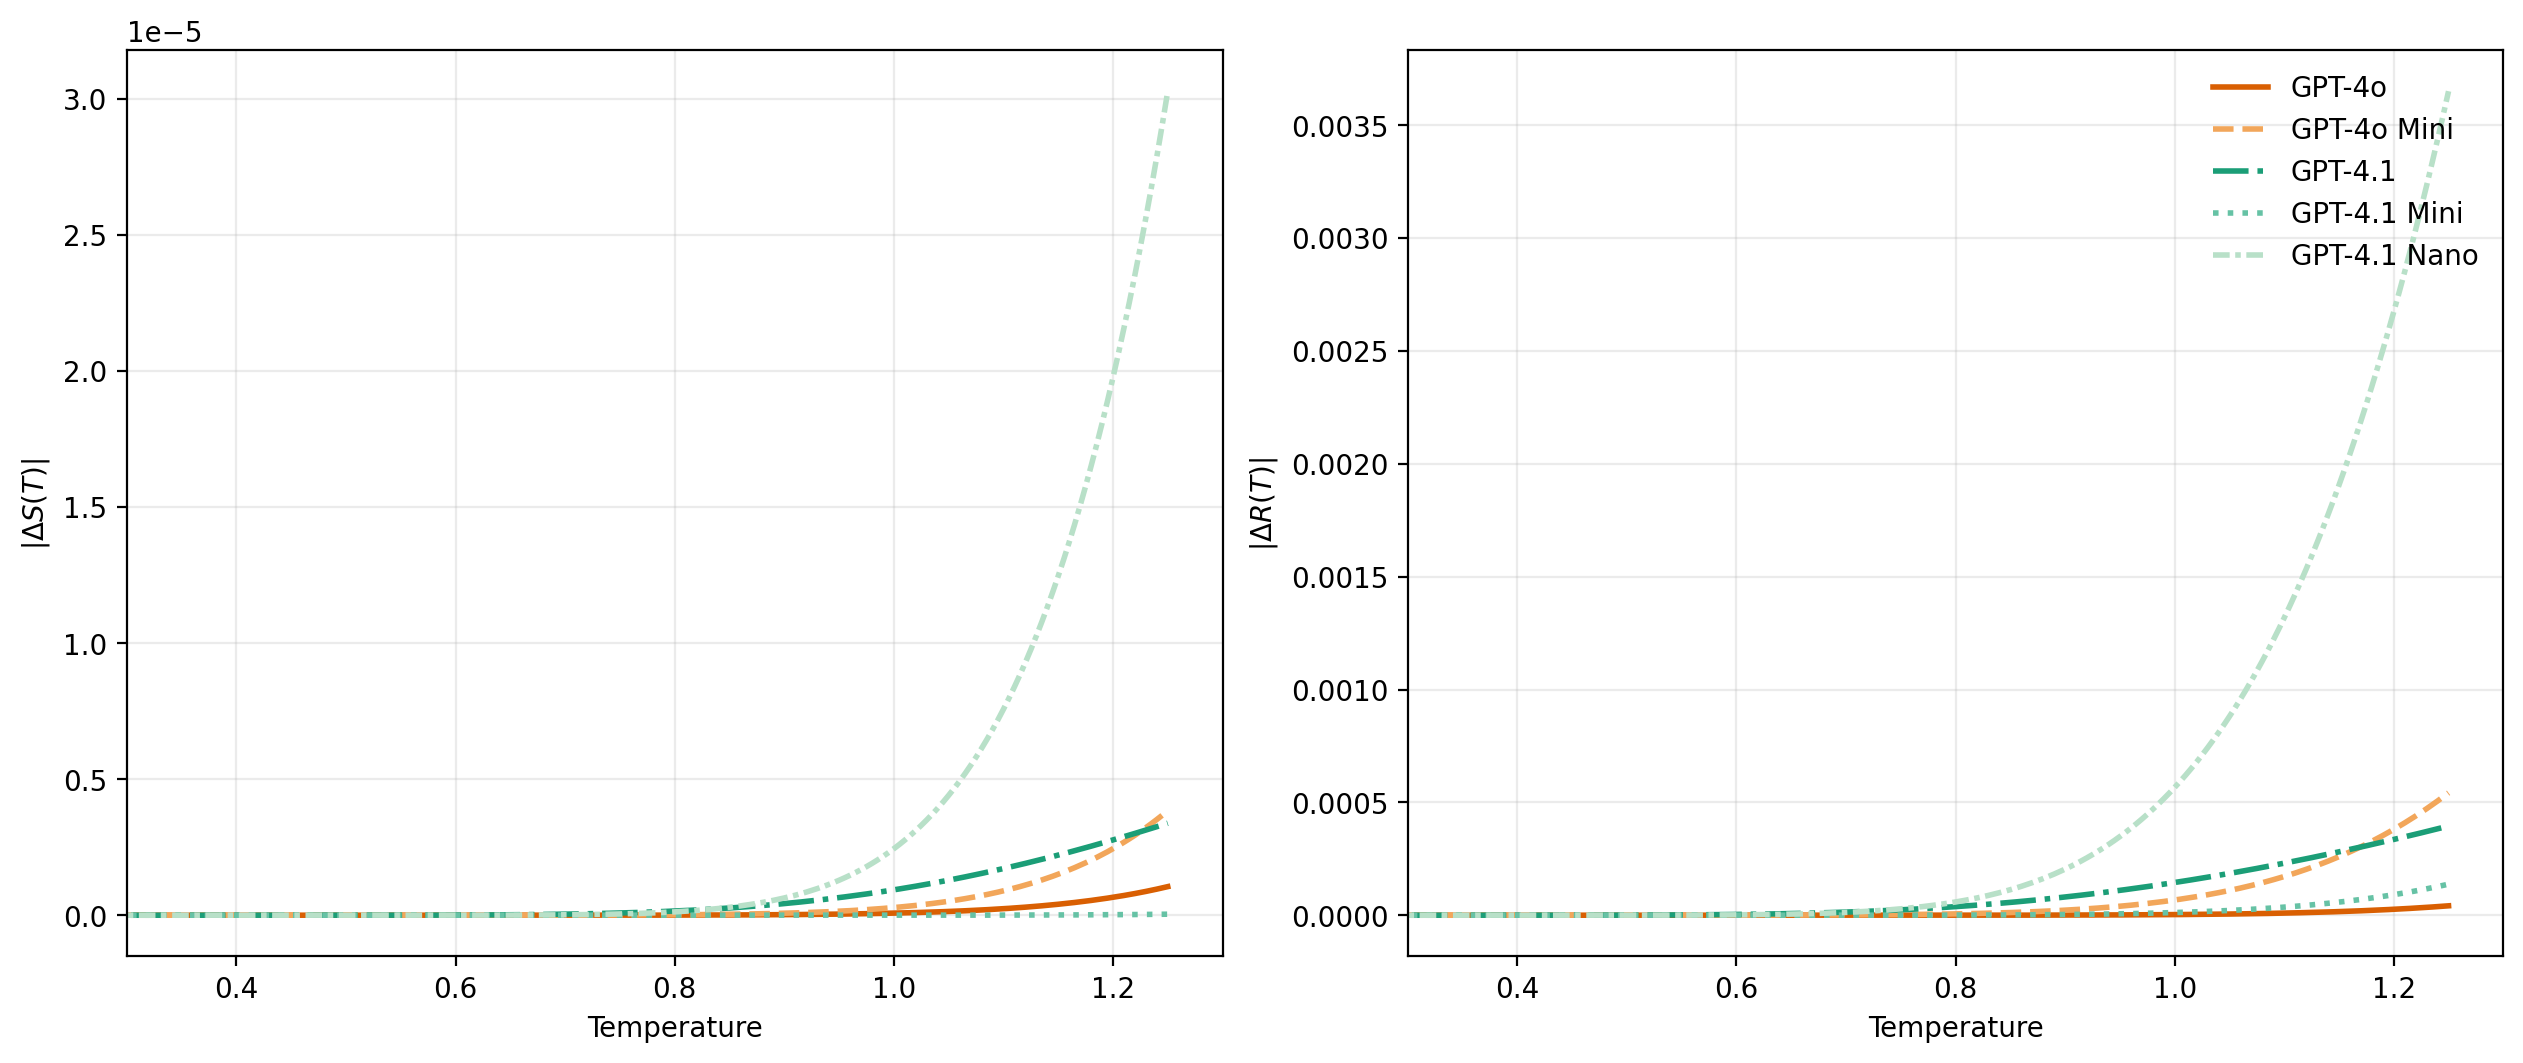
\includegraphics[width=\linewidth]{figures/logprob_imputation_sensitivity.png}
  \caption{Sensitivity of the logit-based temperature curves to the missing-digit imputation rule. We compare the default rule, which assigns every missing digit the minimum returned top-20 log-probability, against a zero-mass alternative. The plotted quantities are the absolute differences in the resulting \(S(T)\) and \(R(T)\) curves. Across all five models and all plotted temperatures, the discrepancies remain very small.}
  \label{fig:logprob-imputation-sensitivity}
\end{figure}



\section{Parsing Failures}
\label{sec:failures}

In the first run, we constrain outputs to begin with a single integer rating from 0 to 5, and parse this leading integer. Parsing failures were recorded and we repeated each attempt multiple times, followed when needed by additional case-by-case recovery that allowed responses not beginning with the rating. In a few cases, models still refused to provide a valid rating for a given persona--question pair after these follow-up attempts. Whenever this happened we excluded these personas from our analysis, because we need a matrix with all valid entries to compute the susceptibility, Eq.~\eqref{eq:overall-susceptibility}.

Persona exclusion is applied per model: any persona for which at least one question cell yields no valid rating is dropped from that model's analysis, since susceptibility requires a complete persona--question mean matrix. For models queried at multiple temperatures, the retained set is additionally intersected across temperatures so that logit-derived curves and sampled data points are computed from the same persona composition; temperature runs with fewer than 50 valid personas are excluded from this intersection. The retained set therefore varies by model.

Table~\ref{tab:failures_by_model} reports, for completeness, the total number of failed parsing rows and failed parsing attempts per model. The difference between the two columns gives a sense of the number of repetitions attempted. We list only models with non-zero totals.

% Auto-generated by analysis/summarize_failures.py
\begin{table}[t]
  \centering
  \caption{Parsing failures per model.}
  \label{tab:failures_by_model}
  \begin{tabular}{lrr}
    \toprule
    Model & Failed rows & Total failures \\
    \midrule
    Claude Haiku 4.5 & 344 & 364 \\
    Claude Sonnet 4.5 & 24 & 37 \\
    DeepSeek V3 & 7 & 7 \\
    DeepSeek V3.1 & 146 & 146 \\
    Gemini 2.5 Flash & 1924 & 1943 \\
    Gemini 2.5 Flash Lite & 129 & 406 \\
    GPT-4.1 & 4 & 4 \\
    GPT-4o & 24 & 37 \\
    GPT-4o Mini & 71 & 202 \\
    Llama 4 Maverick & 27 & 27 \\
    Llama 4 Scout & 16 & 16 \\
    \bottomrule
  \end{tabular}
\end{table}


Some models' responses systematically ignore the leading integer prompt instruction (see Appendix~\ref{app:prompts} for prompt details). In most cases they open with text such as ``As a~\ldots'' before eventually providing a rating. Most cases were model--question specific. However, some personas appeared repeatedly across models, and Table~\ref{tab:uninstructed-personas} highlights the two worst ``offenders" by aggregate parsing failures. This behavior was unexpected as their descriptions (see Appendix~\ref{app:personas}) do not obviously correlate with not following instructions, yet the pattern persists across architectures.

\begin{table}[t!]
  \centering
  \caption{Personas with the highest parsing failure counts.}
  \label{tab:uninstructed-personas}
  \resizebox{\linewidth}{!}{%
  \begin{tabular}{c|ccc|c}
    \toprule
    Persona ID & \texttt{gemini-2.5-flash-lite} & \texttt{gpt-4o} & \texttt{gpt-4o-mini} & Total failures \\
    \midrule
    66 & 30 & 6 & 60 & 96 \\
    94 & 58 & 4 & 30 & 92 \\
    \bottomrule
  \end{tabular}}
\end{table}




\section{Personas}
\label{app:personas}
We evaluated models across a diverse set of personas, denoted as $\mathcal{P}$, to investigate how persona characteristics influence responses on the MFQ. We sampled $|\mathcal{P}| = 100$ personas from prior work on large-scale persona generation \citep{ge2025scalingsyntheticdatacreation}. Each persona description is enumerated below, with the enumeration linking each description to its corresponding persona ID.

\IfFileExists{supplement/appendix_personas.tex}{\input{supplement/appendix_personas}}{\small\emph{Personas list will appear after running the generator script.}}

\end{document}
